\documentclass[lang=cn,newtx,10pt,scheme=chinese]{elegantbook}

\title{计算电磁学}
\subtitle{学习笔记}

\author{曾申昊}
\institute{浙江大学}
\date{\today}
\bioinfo{目标}{完成三种数值方法的学习}

\extrainfo{正在施工中!}

\setcounter{tocdepth}{3}

\logo{logo-blue.png}
\cover{cover.jpg}

% 本文档命令
\usepackage{array}
\newcommand{\ccr}[1]{\makecell{{\color{#1}\rule{1cm}{1cm}}}}

% 修改标题页的橙色带
\definecolor{customcolor}{RGB}{32,178,170}
\colorlet{coverlinecolor}{customcolor}
\usepackage{cprotect}

\addbibresource[location=local]{reference.bib} % 参考文献

\begin{document}

\maketitle
\frontmatter

\tableofcontents

\mainmatter

% 正文内容
\chapter{方程推导}
\chapter{有限差分法}

\section{有限差分公式}

\par 有限差分法要求我们近似微分算子。为了计算函数在 $x$ 点的一阶导数,
我们有三种选择。

\begin{theorem}{前向差分公式}
    \begin{equation}
        f'(x)=\frac{\text{d}f}{\text{d}x}
            \approx\frac{f(x+\Delta x)-f(x)}{\Delta x}
    \end{equation}
\end{theorem}

\begin{theorem}{后向差分公式}
    \begin{equation}
        f'(x)=\frac{\text{d}f}{\text{d}x}
            \approx\frac{f(x)-f(x-\Delta x)}{\Delta x}
    \end{equation}
\end{theorem}

\begin{theorem}{中心差分公式}{一阶导数中心差分公式}
    \begin{equation}
        f'(x)=\frac{\text{d}f}{\text{d}x}
            \approx\frac{f(x+\Delta x)-f(x-\Delta x)}{2\Delta x}
    \end{equation}
\end{theorem}

\par 同样,我们可以用类似的方法来近似二阶导数。

\begin{theorem}{中心差分公式}{二阶导数中心差分公式}
    \begin{equation}
        f''(x)=\frac{\text{d}^2f}{\text{d}x^2}
            \approx
            \frac{f(x+\Delta x)-2f(x)+f(x-\Delta x)}{(\Delta x)^2}
    \end{equation}
\end{theorem}

\begin{exercise}
    证明上述公式,并估计其精度。  
\end{exercise}

\begin{solution}
    基于一个非常朴素的想法,将 $f'(x)$ 代入 
    定理 \ref{thm:一阶导数中心差分公式},就可以得到二阶导数的中心差分公式。
    \begin{align*}
        f''(x)&\approx\frac{f'(x+\frac{\Delta x}{2})-f'(x-\frac{\Delta x}{2})}{\Delta x}\\
        &\approx\frac{\frac{f(x+\Delta x)-f(x)}{\Delta x}
            -\frac{f(x)-f(x-\Delta x)}{\Delta x}}{\Delta x}\\
        &=\frac{f(x+\Delta x)-2f(x)+f(x-\Delta x)}{(\Delta x)^2}
    \end{align*}
    由 Taylor 展开,我们有
    \begin{equation*}
        f(x+\Delta x)=f(x)+f'(x)\Delta x+\frac{f''(x)}{2}(\Delta x)^2
            +\frac{f'''(x)}{6}(\Delta x)^3+\cdots
    \end{equation*}
    \begin{equation*}
        f(x-\Delta x)=f(x)-f'(x)\Delta x+\frac{f''(x)}{2}(\Delta x)^2
            -\frac{f'''(x)}{6}(\Delta x)^3+\cdots
    \end{equation*}
    两式相加,我们有
    \begin{equation*}
        f(x+\Delta x)+f(x-\Delta x)=2f(x)+f''(x)(\Delta x)^2 
        +\mathcal{O}\Big((\Delta x)^4\Big)
    \end{equation*}
    故
    \begin{equation*}
        f''(x)=\frac{f(x+\Delta x)-2f(x)+f(x-\Delta x)}{(\Delta x)^2}
        +\mathcal{O}\Big((\Delta x)^2\Big)
    \end{equation*}
    因此该公式具有二阶精度。
\end{solution}

\par 对于其他差分公式,我们同样可以利用 Taylor 展开来估计精度。

\section{一维问题分析}

\par 以一维波动方程和波动方程为例,简要介绍有限差分法的具体求解操作,
并对其稳定性和数值色散进行分析。

\subsection{扩散方程的求解}

\begin{theorem}{扩散方程}
    当媒质有很大的导体损耗时,其中的传导电流远大于位移电流,因此可忽略位移电流,
    由此得到电场所满足的二阶偏微分方程为
    \begin{equation}
        \nabla \times \nabla \times \vec{\mathscr{E}}
        +\mu \sigma \frac{\partial \vec{\mathscr{E}}}{\partial t}
        =-\mu \frac{\partial \vec{\mathscr{J}_i}}{\partial t}
    \end{equation}
    对于一维情况,假设 $\mathscr{J}_i$ 和 $\mathscr{E}$ 
    只有 $z$ 方向分量且只在 $x$ 方向上有变化,我们有
    \begin{equation}
        \frac{\partial^2 \mathscr{E}_z}{\partial x^2}
        -\mu \sigma \frac{\partial \mathscr{E}_z}{\partial t}
        =\mu \frac{\partial \mathscr{J}_z}{\partial t}
        \label{一维扩散方程}
    \end{equation}
\end{theorem}

\begin{exercise}
    推导上述方程。
\end{exercise}

\begin{definition}
    首先将 $x$ 轴均分成许多小段,记为 $x=i\Delta x$,
    其中 $i=0,1,2,\cdots,M$。类似的,将时间轴均分成许多小段,记为 $t=n\Delta t$,
    其中 $n=0,1,2,\cdots,N$。$\mathscr{E}_z(x,t)$ 可以写为
    \begin{equation}
        \mathscr{E}_z(x,t)=\mathscr{E}_z(i\Delta x,n\Delta t)
        \equiv \mathscr{E}_z^n(i)
    \end{equation}
\end{definition}

\begin{theorem}{时间步进公式}{扩散方程时间步进公式}
    对 $x$ 的二阶导数应用中心差分公式,并对时间的一阶导数应用前向差分公式,我们有
    \begin{equation}
        \mathscr{E}_z^{n+1}(i)=\mathscr{E}_z^n(i)
        +\frac{\Delta t}{\mu \sigma (\Delta x)^2}
        \Big[\mathscr{E}_z^n(i+1)-2\mathscr{E}_z^n(i)+\mathscr{E}_z^n(i-1)\Big]
        -\frac{1}{\sigma}\Big[\mathscr{J}_z^{n+1}(i)-\mathscr{J}_z^{n}(i)\Big]
    \end{equation}
\end{theorem}

\begin{exercise}
    推导上述方程。
\end{exercise}

\begin{solution}
    由式 (\ref{一维扩散方程}),我们有
    \begin{equation*}
        \frac{\partial^2 \mathscr{E}_z}{\partial x^2}
        -\mu \sigma \frac{\partial \mathscr{E}_z}{\partial t}
        =\mu \frac{\partial \mathscr{J}_z}{\partial t}
    \end{equation*}
    对 $x$ 的二阶导数应用中心差分公式,对时间的一阶导数应用前向差分公式,我们有
    \begin{equation*}
        \frac{\mathscr{E}_z^{n}(i+1)-2\mathscr{E}_z^n(i)+\mathscr{E}_z^{n}(i-1)}{(\Delta x)^2}
        -\mu \sigma \frac{\mathscr{E}_z^{n+1}(i)-\mathscr{E}_z^n(i)}{\Delta t}
        =\mu \frac{\mathscr{J}_z^{n+1}(i)-\mathscr{J}_z^n(i)}{\Delta t}
    \end{equation*}
    整理得
    \begin{equation*}
        \mathscr{E}_z^{n+1}(i)=\mathscr{E}_z^n(i)
        +\frac{\Delta t}{\mu \sigma (\Delta x)^2}
        \Big[\mathscr{E}_z^n(i+1)-2\mathscr{E}_z^n(i)+\mathscr{E}_z^n(i-1)\Big]
        -\frac{1}{\sigma}\Big[\mathscr{J}_z^{n+1}(i)-\mathscr{J}_z^{n}(i)\Big]
    \end{equation*}
    由于在时间维上使用的是前向差分公式,所以该公式具有一阶精度。
\end{solution}

\par 为了通过定理 \ref{thm:扩散方程时间步进公式} 求解扩散方程,我们还需要
关于边界条件的信息。通常遇到的边界条件为 Dirichlet 条件和 Neumann 条件。

\begin{theorem}{Dirichlet 条件}
    Dirichlet 条件给定了边界处的场值,如在本例中,$x=0$ 处的值给定为
    \begin{equation}
        \mathscr{E}_z(x=0,t)=p(t)
    \end{equation}
    对于此条件,边界值已知,无须计算。
\end{theorem}

\begin{theorem}{Neumann 条件}
    Neumann 条件规定了边界处的法向导数值,可表示为
    \begin{equation}
        \left.\frac{\partial \mathscr{E}_z(x,t)}{\partial x}\right|_{x=0}=q(t)
    \end{equation}
    使用中心差分离散,其结果为
    \begin{equation}
        \mathscr{E}_z^n(-1)=\mathscr{E}_z^n(1)-2\Delta x q^n
    \end{equation}
    它可以用来计算 $\mathscr{E}_z^{n+1}(0)$。
\end{theorem}

\subsection{波动方程的求解}

\begin{theorem}{波动方程}
    当介质为无耗的时,其电场满足下面的二阶偏微分方程
    \begin{equation}
        \nabla \times \nabla \times \vec{\mathscr{E}}
        +\mu \epsilon \frac{\partial^2 \vec{\mathscr{E}}}{\partial t^2}
        =-\mu \frac{\partial \vec{\mathscr{J}_i}}{\partial t}
    \end{equation}
    对于一维情况,假设 $\mathscr{J}_i$ 和 $\mathscr{E}$ 
    只有 $z$ 方向分量且只在 $x$ 方向上有变化,我们有
    \begin{equation}
        \frac{\partial^2 \mathscr{E}_z}{\partial x^2}
        -\mu \epsilon \frac{\partial^2 \mathscr{E}_z}{\partial t^2}
        =\mu \frac{\partial \mathscr{J}_z}{\partial t}
        \label{一维波动方程}
    \end{equation}
\end{theorem}

\begin{exercise}
    推导上述方程。
\end{exercise}

\begin{theorem}{时间步进公式}{波动方程时间步进公式}
    将空间和时间按照前面描述的方法均匀离散,并对空间和时间导数应用中心差分,则可以
    得到
    \begin{equation}
        \mathscr{E}_z^{n+1}(i)=2\mathscr{E}_z^n(i)-\mathscr{E}_z^{n-1}(i)
        +\frac{(\Delta t)^2}{\mu \epsilon (\Delta x)^2}
        \Big[\mathscr{E}_z^n(i+1)-2\mathscr{E}_z^n(i)+\mathscr{E}_z^n(i-1)\Big]
        -\frac{\Delta t}{2\epsilon}\Big[\mathscr{J}_z^{n+1}(i)-\mathscr{J}_z^{n-1}(i)\Big]
    \end{equation}
\end{theorem}

\begin{exercise}
    推导上述方程。
\end{exercise}

\begin{solution}
    由式 (\ref{一维波动方程}),我们有
    \begin{equation*}
        \frac{\partial^2 \mathscr{E}_z}{\partial x^2}
        -\mu \epsilon \frac{\partial^2 \mathscr{E}_z}{\partial t^2}
        =\mu \frac{\partial \mathscr{J}_z}{\partial t}
    \end{equation*}
    对 $x$ 和时间的二阶导数应用中心差分公式,我们有
    \begin{equation*}
        \frac{\mathscr{E}_z^{n}(i+1)-2\mathscr{E}_z^n(i)+\mathscr{E}_z^{n}(i-1)}{(\Delta x)^2}
        -\mu \epsilon \frac{\mathscr{E}_z^{n+1}(i)-2\mathscr{E}_z^n(i)+\mathscr{E}_z^{n-1}(i)}{(\Delta t)^2}
        =\mu \frac{\mathscr{J}_z^{n+1}(i)-\mathscr{J}_z^{n-1}(i)}{2\Delta t}
    \end{equation*}
    整理得
    \begin{equation*}
        \mathscr{E}_z^{n+1}(i)=2\mathscr{E}_z^n(i)-\mathscr{E}_z^{n-1}(i)
        +\frac{(\Delta t)^2}{\mu \epsilon (\Delta x)^2}
        \Big[\mathscr{E}_z^n(i+1)-2\mathscr{E}_z^n(i)+\mathscr{E}_z^n(i-1)\Big]
        -\frac{\Delta t}{2\epsilon}\Big[\mathscr{J}_z^{n+1}(i)-\mathscr{J}_z^{n-1}(i)\Big]
    \end{equation*}
    由于所有数值微分都使用了中心差分公式,因此该公式具有二阶精度。
\end{solution}

\subsection{稳定性分析}

\par 从前面介绍的扩散方程和波动方程的有限差分公式中不难看出,在有限差分中,需要选
择合适的 $\Delta x$ 和 $\Delta t$,因此必要对时间步进公式进行稳定性分析。

\begin{note}
    通常来说,若关注的最高频率为 $f_{\text{max}}$,
    其相应波长为 $\lambda_{\text{min}}=\frac{c}{f_{\text{max}}}$,
    周期为 $T_{\text{min}}=\frac{1}{f_{\text{max}}}$,
    则 $\Delta x$ 和 $\Delta t$ 的选择应满足
    $\Delta x < \frac{\lambda_{\text{min}}}{20}$ 和
    $\Delta t < \frac{T_{\text{min}}}{20}$。
    当然,这些值的具体选择应根据特定的问题及所需的精度确定。
\end{note}

\par 为了说明稳定性分析的过程,以定理 \ref{thm:扩散方程时间步进公式} 为例。
若丢掉源项,则由能量守恒得知,
求解区域中的场的能量不应该随时间增加。实际上,由于介质损耗,其能量应该减少。这一
点是\textbf{稳定性分析}的基础。

\par 为了考察场的能量,首先把场展开为 Fourier 级数

\begin{equation}
    \mathscr{E}_z^{n}(i)=
    \sum_{m=-\infty}^{\infty}
    A_m^n e^{jk_m i \Delta x}, \qquad k_m = \frac{m\pi}{L}
    \label{场的 Fourier 展开}
\end{equation}

式中,$L=M \Delta x$ 表示求解区域的长度。众所周知,场的能量正比于各 Fourier 模式幅度的平方
和。因此,为了确保能量不随 $n$ 的增加而增加,可以检查 Fourier 模式的幅度。

\begin{definition}
    定义一个放大因子 $g_m$,用于描述场的幅度经过一个时间步长后的变化
    \begin{equation}
        g_m = \frac{A^{n+1}_m}{A^n_m}
    \end{equation}
\end{definition}

\begin{theorem}{稳定性条件}
    为了保证场的能量不随时间增加,对所有 $k_m$,均有 $|g_m| \leq 1$。
    在此条件下,场的能量可保证不会随 $n$ 的增加而增加,因而时间步进过程将是稳定的。
\end{theorem}

\begin{theorem}{扩散方程稳定性条件}{扩散方程稳定性条件}
    对于定理 \ref{thm:扩散方程时间步进公式} 给出的公式,我们有以下稳定性条件
    \begin{equation}
        \Delta t \leq \frac{1}{2} \mu \sigma (\Delta x)^2
    \end{equation}
\end{theorem}

\begin{exercise}
    证明上述稳定性条件。
\end{exercise}

\begin{solution}
    由定理 \ref{thm:扩散方程时间步进公式},我们可以得到其无源项的形式
    \begin{equation*}
        \mathscr{E}_z^{n+1}(i)=\mathscr{E}_z^n(i)
        +\frac{\Delta t}{\mu \sigma (\Delta x)^2}
        \Big[\mathscr{E}_z^n(i+1)-2\mathscr{E}_z^n(i)+\mathscr{E}_z^n(i-1)\Big]
    \end{equation*}
    将其代入式 (\ref{场的 Fourier 展开}),我们有
    \begin{equation*}
        A_m^{n+1}=A_m^n
        +\frac{\Delta t}{\mu \sigma (\Delta x)^2}
        \Big[e^{jk_m \Delta x}-2+e^{-jk_m \Delta x}\Big]A_m^n
    \end{equation*}
    整理得
    \begin{align*}
        g_m&=1
        +\frac{\Delta t}{\mu \sigma (\Delta x)^2}
        \Big[2\cos (k_m \Delta x)-2\Big]\\
        &=1-4\frac{\Delta t}{\mu \sigma (\Delta x)^2}
        \sin^2\left(\frac{k_m \Delta x}{2}\right)\\
        &\in \left[1 - 4\frac{\Delta t}{\mu \sigma (\Delta x)^2}, 1\right]
    \end{align*}
    因此,为保证 $|g_m|\leq 1$,必须有
    \begin{equation*}
        1 - 4\frac{\Delta t}{\mu \sigma (\Delta x)^2} \geq -1
        \quad \text{即} \ 
        \Delta t \leq \frac{1}{2} \mu \sigma (\Delta x)^2
    \end{equation*}
\end{solution}

\begin{theorem}{波动方程稳定性条件}{波动方程稳定性条件}
    对于定理 \ref{thm:波动方程时间步进公式} 给出的公式,我们有以下稳定性条件
    \begin{equation}
        \Delta t \leq \Delta x \sqrt{\mu \epsilon}
    \end{equation}
\end{theorem}

\begin{exercise}
    证明上述稳定性条件。
\end{exercise}

\begin{solution}
    由定理 \ref{thm:波动方程时间步进公式},我们可以得到其无源项的形式
    \begin{equation*}
        \mathscr{E}_z^{n+1}(i)=2\mathscr{E}_z^n(i)-\mathscr{E}_z^{n-1}(i)
        +\frac{(\Delta t)^2}{\mu \epsilon (\Delta x)^2}
        \Big[\mathscr{E}_z^n(i+1)-2\mathscr{E}_z^n(i)+\mathscr{E}_z^n(i-1)\Big]
    \end{equation*}
    将其代入式 (\ref{场的 Fourier 展开}),我们有
    \begin{align*}
        A_m^{n+1}&=2A_m^n-A_m^{n-1}
        +\frac{(\Delta t)^2}{\mu \epsilon (\Delta x)^2}
        \Big[2\cos (k_m \Delta x)-2]A_m^n\\
        &=2A_m^n-A_m^{n-1}
        -4\frac{(\Delta t)^2}{\mu \epsilon (\Delta x)^2}
        \sin^2\left(\frac{k_m \Delta x}{2}\right)A_m^n
    \end{align*}
    我们作以下假设
    \begin{equation*}
        g_m=\frac{A^{n+1}_m}{A^{n}_m}=\frac{A^{n}_m}{A^{n-1}_m}
    \end{equation*}
    代入得
    \begin{gather*}
        g_m=2-\frac{1}{g_m}-4\frac{(\Delta t)^2}{\mu \epsilon (\Delta x)^2}
        \sin^2\left(\frac{k_m \Delta x}{2}\right)\\
        g_m^2-2\alpha_m g_m+1=0 \quad
        \text{其中} \ \alpha_m=1-2\frac{(\Delta t)^2}{\mu \epsilon (\Delta x)^2}\\
        g_m = \alpha_m \pm \sqrt{\alpha_m^2-1}
    \end{gather*}
    因此,为保证 $|g_m|\leq 1$,必须有 $\alpha_m^2 \leq 1$
    \begin{equation*}
        1-2\frac{(\Delta t)^2}{\mu \epsilon (\Delta x)^2} \geq -1
        \quad \text{即} \ 
        \Delta t \leq \Delta x \sqrt{\mu \epsilon}
    \end{equation*}
\end{solution}

\begin{proposition}
    如果在定理 \ref{thm:扩散方程时间步进公式} 中对时间的导数使用中心差分近
    似,我们可以获得二阶精度的时间步进公式,即
    \begin{equation}
        \mathscr{E}_z^{n+1}(i)=\mathscr{E}_z^{n-1}(i)
        +\frac{2\Delta t}{\mu \sigma (\Delta x)^2}
        \Big[\mathscr{E}_z^n(i+1)-2\mathscr{E}_z^n(i)+\mathscr{E}_z^n(i-1)\Big]
        -\frac{1}{\sigma}\Big[\mathscr{J}_z^{n+1}(i)-\mathscr{J}_z^{n-1}(i)\Big]
    \end{equation}
    但该公式在任意步长下都是不稳定的。
\end{proposition}

\begin{exercise}
    证明上述命题。
\end{exercise}

\begin{solution}
    通过相似的推导,我们可以得到
    \begin{equation*}
        g_m^2+2\alpha_m g_m-1=0 \quad \text{其中} 
        \ \alpha_m=\frac{4\Delta t}{\mu \sigma (\Delta x)^2} \sin^2\left(\frac{k_m \Delta x}{2}\right)  
    \end{equation*}
    其解为
    \begin{equation*}
        g_m=-\alpha_m \pm \sqrt{\alpha_m^2+1}
    \end{equation*}
    对于任意 $\alpha_m$,总有$|g_m|>1$,说明该公式总是不稳定的。
\end{solution}

\subsection{数值色散分析}

\par 当有限差分法用于模拟波的传播时,由于数值离散,模拟的波速与波速的物理真实值略
有不同。这将导致波解的相位出现误差,这种现象称为\textbf{数值色散},其造成的误差称为数值相
位误差。

\par 对于一维波动方程,假设平面波沿 $x$ 方向传播,其解析表达式为
\begin{equation}
    \mathscr{E}_z(x,t)=\text{Re}\Big[E_0e^{j(\omega t-kx)}\Big]
\end{equation}
\par 在有限差分网格上,数值离散的波可以表示为
\begin{equation}
    \mathscr{E}^n_z(i)=\text{Re}\Big[E_0e^{j(\omega n \Delta t-\tilde{k} i\Delta x)}\Big]
    \label{数值波解}
\end{equation}

\begin{theorem}{一维数值色散}
    定理 \ref{thm:波动方程时间步进公式} 中给出公式的数值相位误差为
    \begin{equation}
        \frac{\tilde{k}-k}{k}
        \approx\frac{1}{24}\Big[(k\Delta x)^2-(\omega \Delta t)^2\Big]
    \end{equation}
\end{theorem}

\begin{exercise}
    证明上述定理。
\end{exercise}

\begin{solution}
    将式 (\ref{数值波解}) 代入定理 \ref{thm:波动方程时间步进公式} 中的无源项形式
    \begin{equation*}
        \mathscr{E}_z^{n+1}(i)=2\mathscr{E}_z^n(i)-\mathscr{E}_z^{n-1}(i)
        +\frac{(\Delta t)^2}{\mu \epsilon (\Delta x)^2}
        \Big[\mathscr{E}_z^n(i+1)-2\mathscr{E}_z^n(i)+\mathscr{E}_z^n(i-1)\Big]
    \end{equation*}
    我们有
    \begin{equation*}
        \mathscr{E}_z^{n+1}(i)+\mathscr{E}_z^{n-1}(i)=2\mathscr{E}_z^n(i)
        -2\frac{(\Delta t)^2}{\mu \epsilon (\Delta x)^2}\mathscr{E}_z^n(i)
        +\frac{(\Delta t)^2}{\mu \epsilon (\Delta x)^2}
        \Big[\mathscr{E}_z^n(i+1)+\mathscr{E}_z^n(i-1)\Big]
    \end{equation*}
    \begin{equation*}
        \left\{
            \begin{aligned}
                \text{LHS}&=\text{Re}\Big[E_0e^{j(\omega n \Delta t-\tilde{k} i\Delta x)}\Big]
                2\cos(\omega\Delta t)\\
                \text{RHS}&=\text{Re}\Big[E_0e^{j(\omega n \Delta t-\tilde{k} i\Delta x)}\Big]
                \left[2-2\frac{(\Delta t)^2}{\mu \epsilon (\Delta x)^2}+2\frac{(\Delta t)^2}{\mu \epsilon (\Delta x)^2}
                \cos(\tilde{k}\Delta x)\right]
            \end{aligned}
        \right.
    \end{equation*}
    整理得
    \begin{equation*}
        \cos(\omega \Delta t)=(1-r)+r\cos(\tilde{k}\Delta x) 
        \quad \text{其中} \ r=\frac{(\Delta t)^2}{\mu \epsilon (\Delta x)^2}
    \end{equation*}
    解方程可得到数值波数的精确解
    \begin{equation*}
        \tilde{k}=\frac{1}{\Delta x}
        \arccos \left(1-\frac{2}{r}\sin^2 \frac{\omega \Delta t}{2}\right)
    \end{equation*}
    为了得到更明确的表达式,可把余弦函
    数用级数展开式的前三项近似表示,得到
    \begin{gather*}
        1-\frac{1}{2}(\omega \Delta t)^2+\frac{1}{24}(\omega \Delta t)^4
        \approx (1-r)+r\left(1-\frac{1}{2}(\tilde{k} \Delta x)^2
        +\frac{1}{24}(\tilde{k} \Delta x)^4\right)\\
        -\frac{1}{2}(\omega \Delta t)^2+\frac{1}{24}(\omega \Delta t)^4
        \approx r\left(-\frac{1}{2}(\tilde{k} \Delta x)^2
        +\frac{1}{24}(\tilde{k} \Delta x)^4\right)\\
        k^2-\frac{1}{12}k^2(\omega \Delta t)^2 \approx
        \tilde{k}^2-\frac{1}{12}\tilde{k}^2(\tilde{k} \Delta x)^2\\
        \frac{\tilde{k}-k}{k}
        \approx\frac{1}{24}\Big[(k\Delta x)^2-(\omega \Delta t)^2\Big]
    \end{gather*}
\end{solution}

\begin{example}
    若选择 $\Delta t = \Delta x \sqrt{\mu \epsilon}$,
    则数值波数 $\tilde{k}$ 将与波数真实值 $k$ 相同。
\end{example}

\begin{example}
    若选择 $\Delta t = 0.5 \Delta x \sqrt{\mu \epsilon}$,这两个波数之间将有微小的差别
    \begin{equation*}
        \frac{\tilde{k}-k}{k}
        \approx\frac{1}{32}(k \Delta x)^2
        =\frac{\pi^2}{8}\left(\frac{\Delta x}{\lambda}\right)^2
    \end{equation*}
    上式表明此误差随着 $\frac{\Delta x}{\lambda}$ 二次衰减,误差二阶收敛。
\end{example}

\begin{note}
    另外需要指出,一维的波传播是一个特殊问题,因为此时的波传播方向是固定的。在这种
情况下,我们总是可以选择适当的 $\Delta t$,以消除相位误差。而对于二维和三维的问题,情况则完
全不同,此时的波传播方向通常是未知的且随空间位置而变化,因此一般不能通过调整 $\Delta t$ 来消
除相位误差。
\end{note}

\section{二维分析}

\subsection{时域分析}

\begin{theorem}{电场方程}{二维时域电场方程}
    一般情形下,电场所满足的二阶微分方程为
    \begin{equation}
        \nabla \times \nabla \times \vec{\mathscr{E}}
        +\mu \epsilon \frac{\partial^2 \vec{\mathscr{E}}}{\partial t^2}
        +\mu \sigma \frac{\partial \vec{\mathscr{E}}}{\partial t}
        =-\mu \frac{\partial \vec{\mathscr{J}_i}}{\partial t}
    \end{equation}
    对于二维情况,假设源和媒质沿轴是均匀的,
    因此源所产生的场在 $z$ 方向上没有变化。
    若源是 $z$ 方向的电流源,则其产生的电场只有 $z$ 分量。
    由此,我们有
    \begin{equation}
        \frac{\partial^2 \mathscr{E}_z}{\partial x^2}
        +\frac{\partial^2 \mathscr{E}_z}{\partial y^2}
        -\mu \epsilon \frac{\partial^2 \mathscr{E}_z}{\partial t^2}
        -\mu \sigma \frac{\partial \mathscr{E}_z}{\partial t}
        =\mu \frac{\partial \mathscr{J}_z}{\partial t}
        \label{二维电场方程}
    \end{equation}
\end{theorem}

\begin{definition}
    将求解区域用矩形框围住,再把它划分成尺寸为 $\Delta x \times \Delta y$ 的许多小矩形,
    每个网格点可以用一对整数 $(i,j)$ 表示。类似一维情形,我们作以下简写
    \begin{equation}
        \mathscr{E}_z(x,y,t)=\mathscr{E}_z(i\Delta x,j\Delta y,n\Delta t)
        \equiv \mathscr{E}_z^n(i,j)
    \end{equation}
\end{definition}

\begin{theorem}{时间步进公式}{二维扩散方程时间步进公式}
    对 $x$ 和 $y$ 的二阶导数应用中心差分公式,对时间的一阶和二阶导数应用中心差分公式,我们有
    \begin{equation}
        \begin{aligned}
            \mathscr{E}_z^{n+1}(i,j)=
            &\left[\frac{\mu\sigma_{ij}}{2\Delta t}+\frac{\mu\epsilon_{ij}}{(\Delta t)^2}\right]^{-1}
            \Bigg\{2\mathscr{E}_z^n(i,j)\left[
                \frac{\mu\epsilon_{ij}}{(\Delta t)^2}
                -\frac{1}{(\Delta x)^2}-\frac{1}{(\Delta y)^2}
            \right]\\
            &+\mathscr{E}_z^{n-1}(i,j)\left[
                \frac{\mu\sigma_{ij}}{2\Delta t}-\frac{\mu\epsilon_{ij}}{(\Delta t)^2}
            \right]
            +\frac{1}{(\Delta x)^2}\Big[\mathscr{E}_z^{n}(i+1,j)+\mathscr{E}_z^{n}(i-1,j)\Big]\\
            &+\frac{1}{(\Delta y)^2}\Big[\mathscr{E}_z^{n}(i,j+1)+\mathscr{E}_z^{n}(i,j-1)\Big]\\
            &-\frac{\mu}{2\Delta t}\Big[\mathscr{J}_z^{n+1}(i,j)-\mathscr{J}_z^{n-1}(i,j)\Big]\Bigg\}
        \end{aligned}
    \end{equation}
\end{theorem}

\begin{exercise}
    推导上述方程。
\end{exercise}

\begin{solution}
    由式 (\ref{二维电场方程}),我们有
    \begin{equation*}
        \frac{\partial^2 \mathscr{E}_z}{\partial x^2}
        +\frac{\partial^2 \mathscr{E}_z}{\partial y^2}
        -\mu \epsilon \frac{\partial^2 \mathscr{E}_z}{\partial t^2}
        -\mu \sigma \frac{\partial \mathscr{E}_z}{\partial t}
        =\mu \frac{\partial \mathscr{J}_z}{\partial t}
    \end{equation*}
    对 $x$ 和 $y$ 的二阶导数应用中心差分公式,对时间的一阶和二阶导数应用中心差分公式,我们有
    \begin{equation*}
        \begin{gathered}
            \frac{\mathscr{E}_z^{n}(i+1,j)-2\mathscr{E}_z^n(i,j)+\mathscr{E}_z^{n}(i-1,j)}{(\Delta x)^2}
            +\frac{\mathscr{E}_z^{n}(i,j+1)-2\mathscr{E}_z^n(i,j)+\mathscr{E}_z^{n}(i,j-1)}{(\Delta y)^2}\\
            -\mu \epsilon_{ij} \frac{\mathscr{E}_z^{n+1}(i,j)-2\mathscr{E}_z^n(i,j)+2\mathscr{E}_z^{n-1}(i,j)}{(\Delta t)^2}
            -\mu \sigma_{ij} \frac{\mathscr{E}_z^{n+1}(i,j)-\mathscr{E}_z^{n-1}(i,j)}{2\Delta t}\\
            =\mu \frac{\mathscr{J}_z^{n+1}(i)-\mathscr{J}_z^{n-1}(i)}{2\Delta t}
        \end{gathered}
    \end{equation*}
    整理后可得到时间步进公式。由于所有数值微分都使用了中心差分公式,因此该公式具有二阶精度。
\end{solution}

\begin{theorem}{稳定性条件}
    对于定理 \ref{thm:二维扩散方程时间步进公式} 给出的公式,我们有以下稳定性条件
    \begin{equation}
        \Delta t \leq \frac{\sqrt{\mu \epsilon}}
        {\sqrt{\frac{1}{(\Delta x)^2}+\frac{1}{(\Delta y)^2}}}
    \end{equation}
\end{theorem}

\begin{exercise}
    证明上述定理。
\end{exercise}

\begin{theorem}{二维数值色散}
    对于定理 \ref{thm:二维扩散方程时间步进公式} 给出的公式,其数值相位误差为
    \begin{equation}
        \frac{\tilde{k}-k}{k}
        \approx\frac{1}{24}
        \Big[(k\Delta x)^2\cos^4\phi^i+(k\Delta y)^2\sin^4\phi^i-(\omega \Delta t)^2\Big]
    \end{equation}
    其中 $\phi^i$ 为波传播方向与 $x$ 轴的夹角。
\end{theorem}

\begin{exercise}
    证明上述定理。
\end{exercise}

\begin{example}
    若选择 $\Delta x=\Delta y = h$ 和 $\Delta t = \frac{0.5h}{c}$,则数值相位误差为
    \begin{equation*}
        \frac{\tilde{k}-k}{k}
        \approx\frac{(kh)^2}{24}
        \left[\cos^4\phi^i+\sin^4\phi^i-\frac{1}{4}\right]
        =\frac{\pi^2}{24}\left(\frac{h}{\lambda}\right)^2\Big[2+\cos(4\phi^i)\Big]
    \end{equation*}
    显然,此相位误差是传播角度的函数。当波沿对角线方向传播时,该误差最小。
\end{example}

\subsection{频域分析}

\par 有限差分法也可以用于求解频域 Maxwell 方程组。

\begin{theorem}{电场方程}{二维频域电场方程}
    对定理 \ref{thm:二维时域电场方程} 中给出的公式作 Fourier 变化,
    可以得到电场满足的频域表达式
    \begin{equation}
        \nabla \times \nabla \times \vec{E}
        -\omega^2\mu \epsilon  \vec{E}
        +j\omega \mu \sigma \vec{E}
        =-j\omega\mu \vec{J_i}
    \end{equation}
    对于二维情况,对源和媒质作与上述定理中同样的假设,我们有
    \begin{equation}
        \frac{\partial^2 E_z}{\partial x^2}
        +\frac{\partial^2 E_z}{\partial y^2}
        +\omega^2\mu \epsilon  E_z
        -j\omega \mu \sigma E_z
        =j\omega\mu J_z
        \label{二维频域电场方程}
    \end{equation}
    定义记号 $g=j\omega \mu J_z$ 和 $\epsilon_c=1-\frac{j\sigma}{\omega \epsilon}$,
    方程可简化为
    \begin{equation}
        \frac{\partial^2 E_z}{\partial x^2}
        +\frac{\partial^2 E_z}{\partial y^2}
        +k^2\epsilon_c  E_z
        =g
    \end{equation}
\end{theorem}

\begin{exercise}
    推导上述方程。
\end{exercise}

\begin{theorem}
    对于定理 \ref{thm:二维频域电场方程} 给出的公式作中心差分可以得到五点差分格式的方程
    \begin{equation}
        \begin{gathered}
            \frac{E_z(i+1,j)-2E_z(i,j)+E_z(i-1,j)}{(\Delta x)^2}
            +\frac{E_z(i,j-1)-2E_z(i,j)+E_z(i,j+1)}{(\Delta y)^2}\\
            +k^2\epsilon_c E_z(i,j)
            =g(i,j)
        \end{gathered}
        \label{二维频域电场方程差分格式}
    \end{equation}
\end{theorem}

\par 对于每个网格点,我们都可以得到类似的方程,其场值均可以采用
式 (\ref{二维频域电场方程差分格式}) 表示。由此得到一组
线性方程组,在给定的边界条件下同时求解整个线性方程组,即可求得网格点的场值。

\begin{note}
    由于 Fourier 变换消除了时间变量,因此我们得到的是一个仅和位置有关的式子,
    可以直接求解线性方程组,而不需要通过时间步进公式迭代。
\end{note}

\par 线性方程组的求解一般有两类方法。
\begin{itemize}
    \item 直接法
    \begin{itemize}
        \item Gauss 消元法
        \item LU 分解法
        \item Cholesky 分解法
    \end{itemize}
    \item 迭代法
    \begin{itemize}
        \item Jacobi 迭代法
        \item Gauss-Seidel 迭代法
        \item SOR 迭代法
        \item 共轭梯度法
    \end{itemize}
\end{itemize}

\section{Yee 网格}

\par 虽然上节中所描述的有限差分法拓展到三维问题会遇到一些严重的问题。这些问题的产生来自于传统的有限差分法在网格点的采
样。

\begin{itemize}
    \item 当网格点位于两种不同媒质的分界面上时,为了保证切向场的连续和法向场的不连续,
    需要进行相当烦琐的处理。
    \item 当一个网格点位于导体或媒质的边缘
    或拐角时,这一点的法向没有明确的定义,而其场分量可能是无限大的,即奇异的,因此这
    个网格点处的场值无法精确描述。
\end{itemize}

\par 而 Yee 网格作为一种独特的离散方法,成功地解
决了这些问题。

\subsection{二维分析}

\begin{theorem}
    重新考虑二维电磁问题。对于源为 $\vec{\mathscr{J}_i}=\vec{z}\mathscr{J}_z$
    的二维问题,其 Maxwell 方程组可简化为
    \begin{align}
        \label{Yee Maxwell 方程组-1}
        \frac{\partial \mathscr{E}_z}{\partial y}
        &= -\mu \frac{\partial \mathscr{H}_x}{\partial t}\\
        \label{Yee Maxwell 方程组-2}
        \frac{\partial \mathscr{E}_z}{\partial x}
        &= \mu \frac{\partial \mathscr{H}_y}{\partial t}\\
        \label{Yee Maxwell 方程组-3}
        \frac{\partial \mathscr{H}_y}{\partial x}
        -\frac{\partial \mathscr{H}_x}{\partial y}
        &= \epsilon \frac{\partial \mathscr{E}_z}{\partial t}
        +\sigma \mathscr{E}_z + \mathscr{J}_z
    \end{align}
\end{theorem}

\par 把求解区域围在一个矩形区域内,然后把区域均匀离散成许多
小矩形单元。每个单元的中心用一对整数 $(i,j)$ 表示,在这个点上采样
$\mathscr{E}_z$。而磁场分量则沿着矩形单元的边缘采样。
通过在 $t=n\Delta t$ 时刻采样电
场,而在 $t=\left(n+\frac{1}{2}\right)\Delta t$ 时刻采样磁场。

\begin{figure}[!htbp]
    \centering
    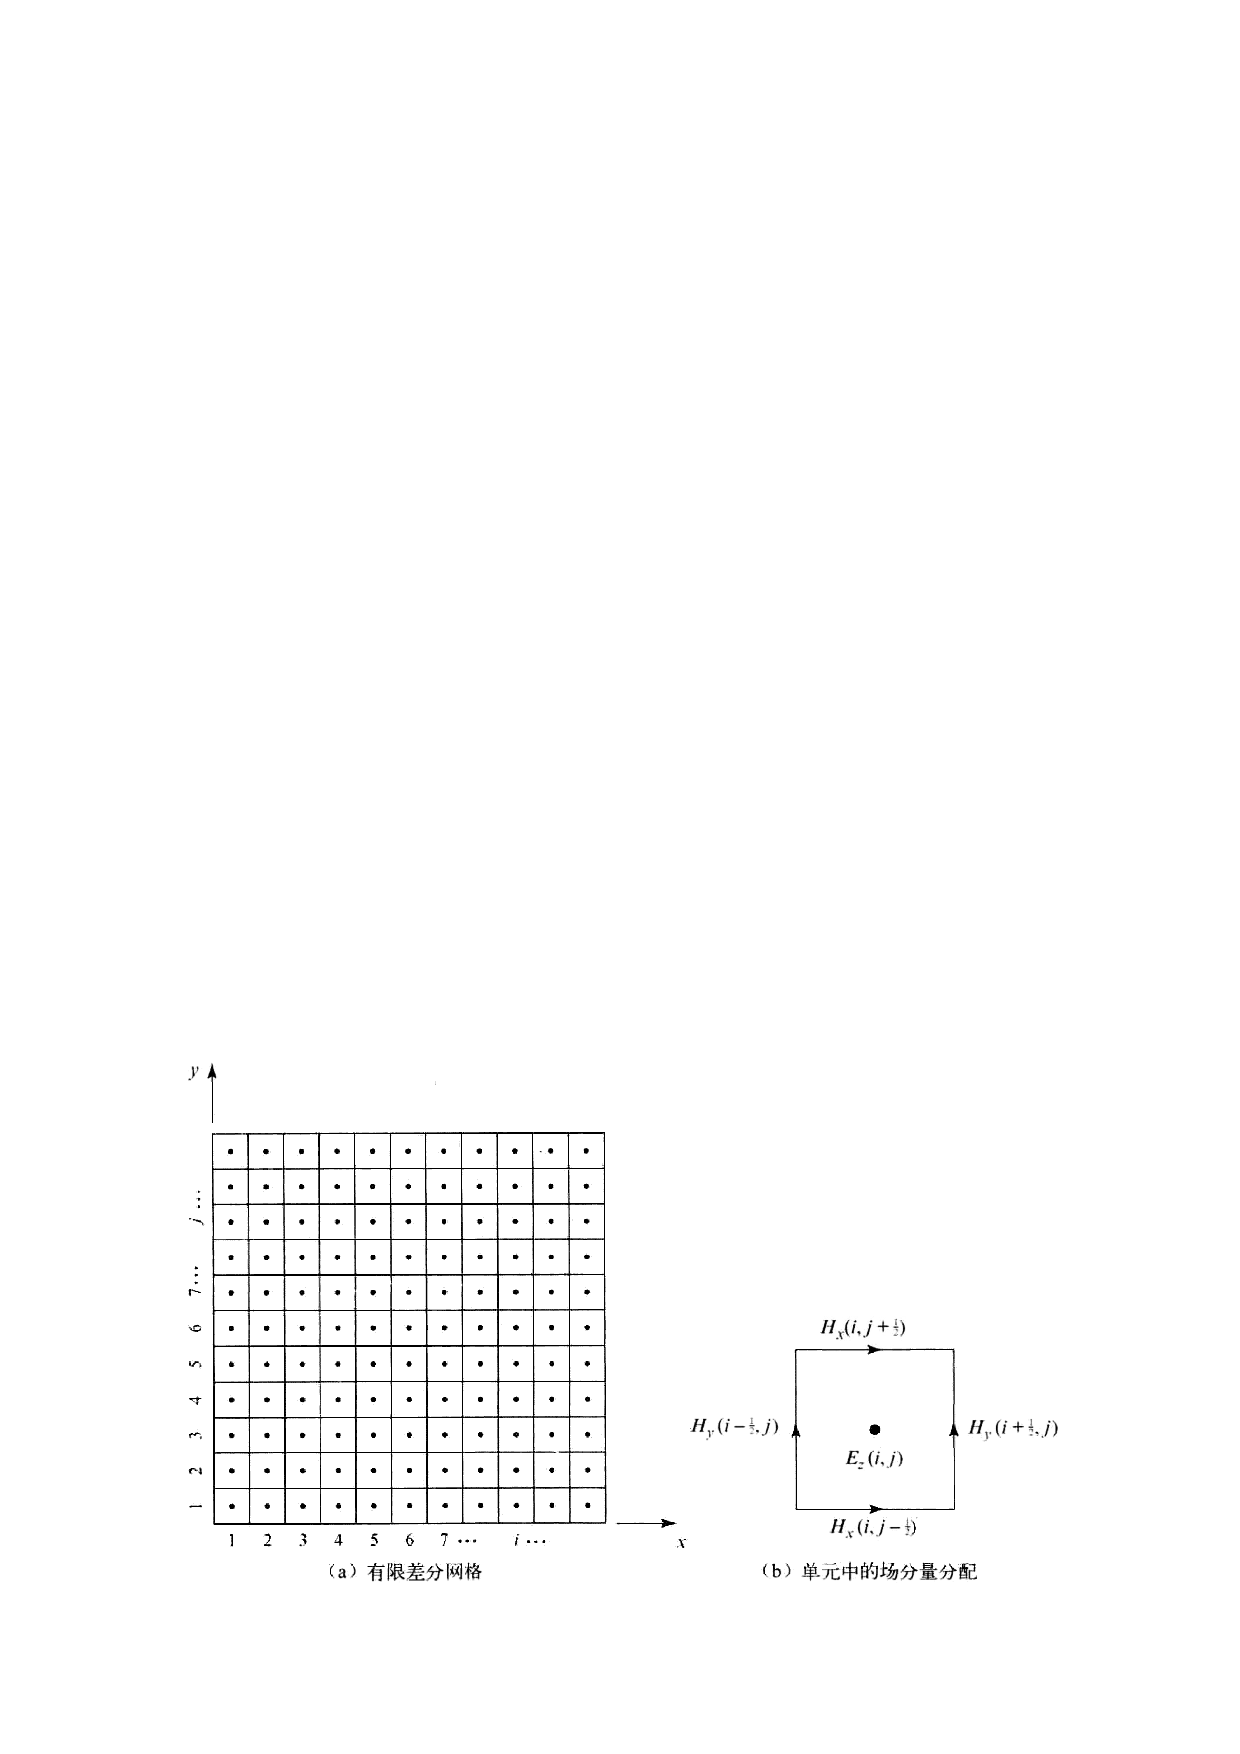
\includegraphics[scale=1]{2.4.1-1.pdf}
    \caption{Yee 网格有限差分算法}
\end{figure}

\begin{theorem}
    对于 Yee 网格,
    式 (\ref{Yee Maxwell 方程组-1}),式 (\ref{Yee Maxwell 方程组-2}) 
    和式 (\ref{Yee Maxwell 方程组-3})
    的时间步进公式分别为
    \begin{equation}
        \mathscr{H}_x^{n+\frac{1}{2}}\left(i,j+\frac{1}{2}\right)=
        \mathscr{H}_x^{n-\frac{1}{2}}\left(i,j+\frac{1}{2}\right)
        -\frac{\Delta t}{\mu \Delta y}\Big[
        \mathscr{E}_z^n(i,j+1)-\mathscr{E}_z^n(i,j)
        \Big]
        \label{Yee 时间步进公式-1}
    \end{equation}
    \begin{equation}
        \mathscr{H}_y^{n+\frac{1}{2}}\left(i+\frac{1}{2},j\right)=
        \mathscr{H}_y^{n-\frac{1}{2}}\left(i+\frac{1}{2},j\right)
        -\frac{\Delta t}{\mu \Delta y}\Big[
        \mathscr{E}_z^n(i+1,j)-\mathscr{E}_z^n(i,j)
        \Big]
        \label{Yee 时间步进公式-2}
    \end{equation}
    \begin{equation}
        \begin{aligned}
            \mathscr{E}_z^{n+1}(i,j)=&\ \frac{1}{\beta(i,j)}
            \Bigg\{\alpha(i,j)\mathscr{E}_z^n(i,j)+\frac{1}{\Delta x}\left[
                \mathscr{H}_y^{n+\frac{1}{2}}\left(i+\frac{1}{2},j\right)
                -\mathscr{H}_y^{n+\frac{1}{2}}\left(i-\frac{1}{2},j\right)
            \right]\\
            &-\frac{1}{\Delta y}
            \left[\mathscr{H}_x^{n+\frac{1}{2}}\left(i,j+\frac{1}{2}\right)
            -\mathscr{H}_x^{n+\frac{1}{2}}\left(i,j-\frac{1}{2}\right)
            \right]-\mathscr{J}_z^{n+\frac{1}{2}}(i,j)
            \Bigg\}
        \end{aligned}
        \label{Yee 时间步进公式-3}
    \end{equation}
    其中 $\alpha(i,j)=\frac{\epsilon}{\Delta t}-\frac{\sigma}{2}$,
    $\beta(i,j)=\frac{\epsilon}{\Delta t}+\frac{\sigma}{2}$。
\end{theorem}

\begin{exercise}
    推导上述方程。
\end{exercise}

\begin{solution}
    以式 (\ref{Yee Maxwell 方程组-1}) 为例,对时间采用中心差分,我们有
    \begin{equation*}
        \frac{\mathscr{E}_z^n(i,j+1)-\mathscr{E}_z^n(i,j)}{\Delta y}
        =-\mu \frac{\mathscr{H}_x^{n+\frac{1}{2}}\left(i,j+\frac{1}{2}\right)
        -\mathscr{H}_x^{n-\frac{1}{2}}\left(i,j+\frac{1}{2}\right)}{\Delta t}
    \end{equation*}
    整理得
    \begin{equation*}
        \mathscr{H}_x^{n+\frac{1}{2}}\left(i,j+\frac{1}{2}\right)=
        \mathscr{H}_x^{n-\frac{1}{2}}\left(i,j+\frac{1}{2}\right)
        -\frac{\Delta t}{\mu \Delta y}\Big[
        \mathscr{E}_z^n(i,j+1)-\mathscr{E}_z^n(i,j)
        \Big]
    \end{equation*}
\end{solution}

\par 对于给定 $\mathscr{E}_z$、$\mathscr{H}_x$ 
及 $\mathscr{H}_y$ 的初值和适当的边界条件,
可以用式 (\ref{Yee 时间步进公式-1}) 和式 (\ref{Yee 时间步进公式-2}) 计
算 $\mathscr{H}_x$ 
和 $\mathscr{H}_y$,然后用式 (\ref{Yee 时间步进公式-3}) 计算
$\mathscr{E}_z$。

\begin{note}
    Yee 网格的一个重要特点是,场和磁场的空间网格错开
    了半个网格点,在时间采样点上也错开半个时间步。
    更重要的是,磁场分量的采样在矩形单
    元的边缘:$\mathscr{H}_x$ 在与 $x$ 平行的边缘上采样;
    $\mathscr{H}_y$ 在与 $y$ 平行的边缘上采样。这种采样方式保证
    了场的唯一定义,并且自动确保了切向场的连续性。
\end{note}

\par 基于式 (\ref{Yee 时间步进公式-1})
和式 (\ref{Yee 时间步进公式-2}) 的时间步进公式称为蛙跳时间积分。

\begin{exercise}
    从积分形式的 Maxwell 方程组出发,推导 Yee 网格的时间步进公式。
\end{exercise}

\subsection{三维分析}

\par Yee 网格有限差分算法可直接从二维扩展到三维。

\begin{theorem}
    考虑时域 Maxwell 方程组
    \begin{align}
        \nabla \times \vec{\mathscr{E}} &= -\mu \frac{\partial \vec{\mathscr{H}}}{\partial t}\\
        \nabla \times \vec{\mathscr{H}} &= 
        \epsilon \frac{\partial \vec{\mathscr{E}}}{\partial t}
        +\sigma \vec{\mathscr{E}}
        +\vec{\mathscr{J}_i}
    \end{align}
    这两个矢量方程可以写成 6 个标量方程
    \begin{align}
        \frac{\partial \mathscr{E}_z}{\partial y}
        -\frac{\partial \mathscr{E}_y}{\partial z}
        &= -\mu \frac{\partial \mathscr{H}_x}{\partial t}\\
        \frac{\partial \mathscr{E}_x}{\partial z}
        -\frac{\partial \mathscr{E}_z}{\partial x}
        &= -\mu \frac{\partial \mathscr{H}_y}{\partial t}\\
        \frac{\partial \mathscr{E}_y}{\partial x}
        -\frac{\partial \mathscr{E}_x}{\partial y}
        &= -\mu \frac{\partial \mathscr{H}_z}{\partial t}\\
        \frac{\partial \mathscr{H}_z}{\partial y}
        -\frac{\partial \mathscr{H}_y}{\partial z}
        &= \epsilon \frac{\partial \mathscr{E}_x}{\partial t}
        +\sigma \mathscr{E}_x + \mathscr{J}_x\\
        \frac{\partial \mathscr{H}_x}{\partial z}
        -\frac{\partial \mathscr{H}_z}{\partial x}
        &= \epsilon \frac{\partial \mathscr{E}_y}{\partial t}
        +\sigma \mathscr{E}_y + \mathscr{J}_y\\
        \frac{\partial \mathscr{H}_y}{\partial x}
        -\frac{\partial \mathscr{H}_x}{\partial y}
        &= \epsilon \frac{\partial \mathscr{E}_z}{\partial t}
        +\sigma \mathscr{E}_z + \mathscr{J}_z
    \end{align}
\end{theorem}

\par 用一个立方体包围体积 $V$,再把这
个立方体盒子分成许多小立方体单元。然后,在单元每条边的中心位置
对电场分量采样,在单元每个面的中心位置对磁场分量采样。若将整个
网格在每个方向上偏移半个单元,则磁场分量的采样点将在单元每条边的中心,而电场分量
的采样点将在单元每个面的中心。

\begin{figure}[!htbp]
    \centering
    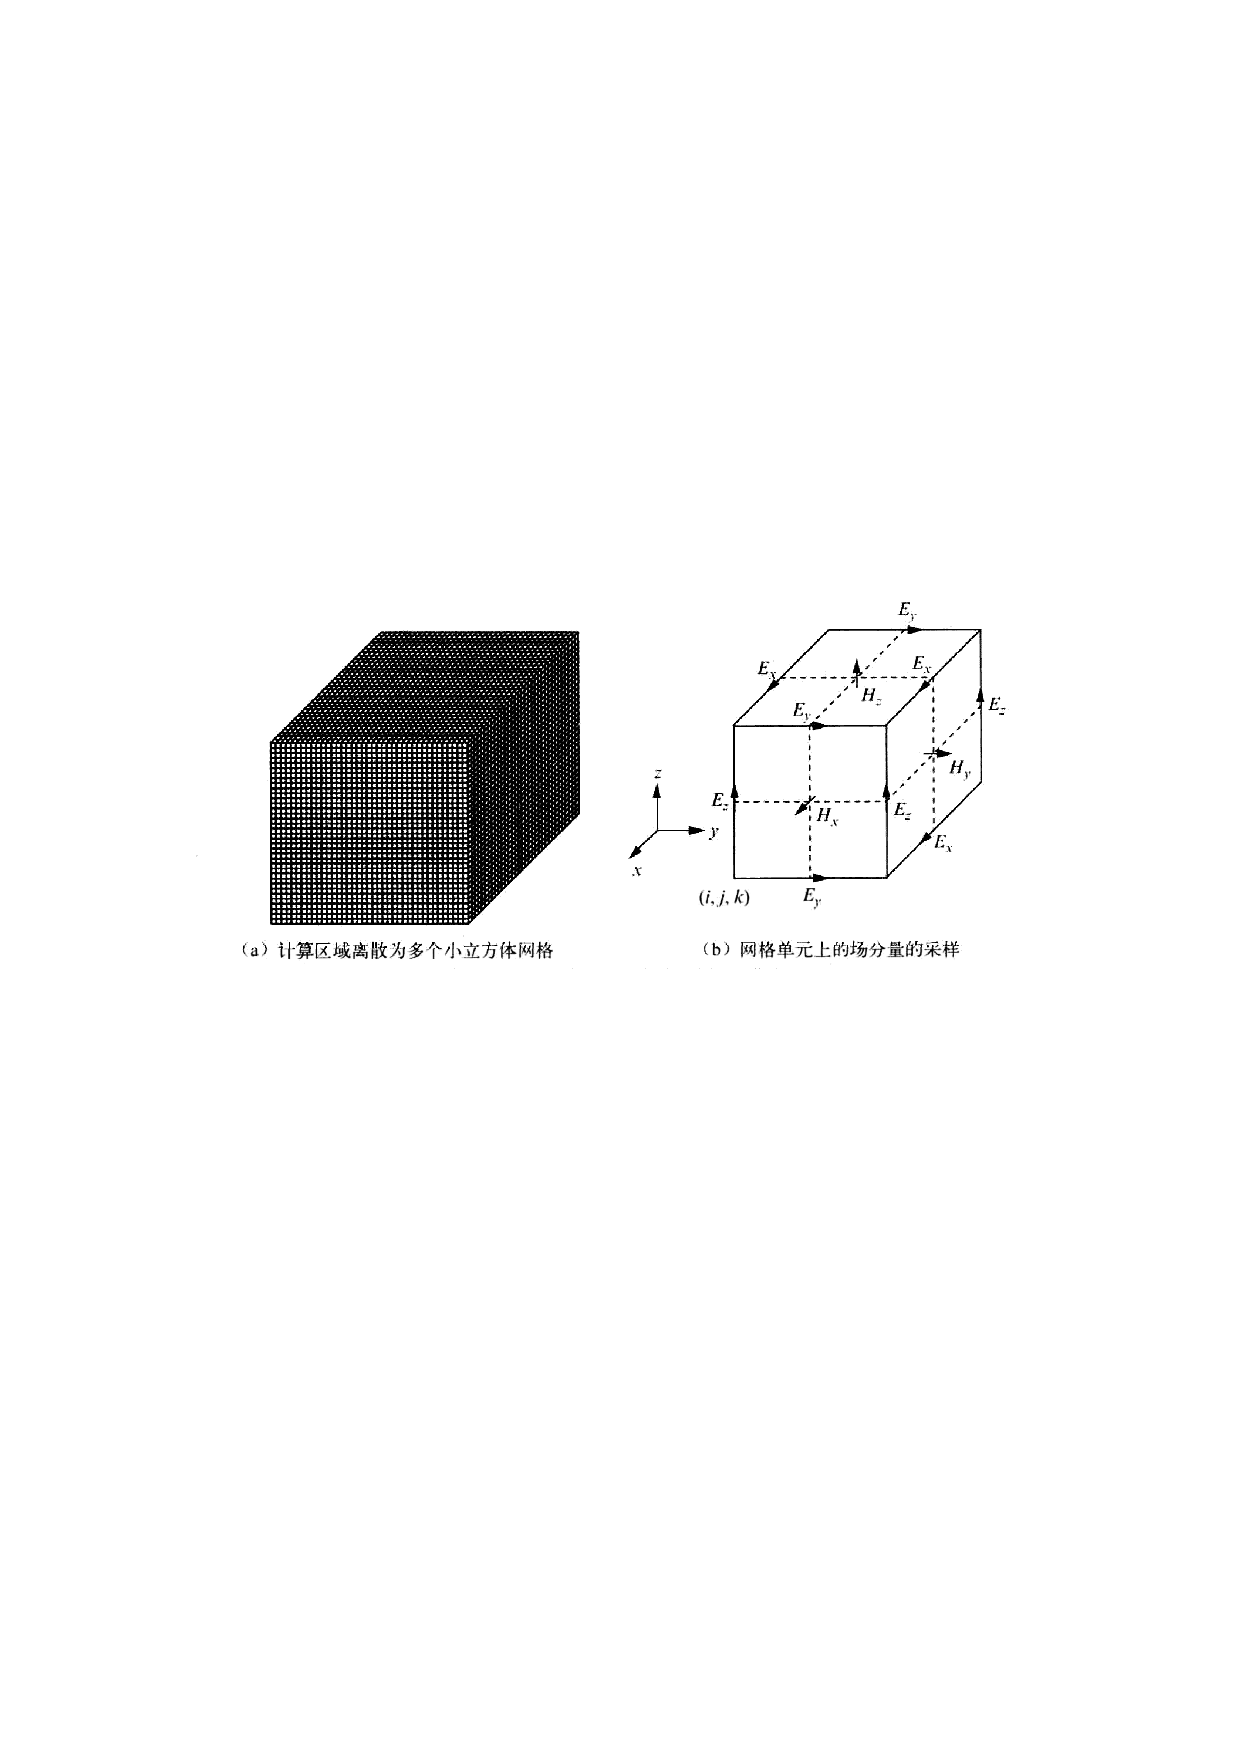
\includegraphics[scale=1]{2.4.2-1.pdf}
    \caption{Yee 网格有限差分算法}
\end{figure}

\begin{theorem}
    待完成
\end{theorem}

\begin{theorem}{稳定性条件}
    保证时间步进的稳定性,其时间步长应满足稳定性条件
    \begin{equation}
        \Delta t \leq \frac{\sqrt{\mu \epsilon}}
        {\sqrt{\frac{1}{(\Delta x)^2}+\frac{1}{(\Delta y)^2}+\frac{1}{(\Delta z)^2}}}
    \end{equation}
\end{theorem}

\begin{theorem}{三维数值色散}
    将数值色散误差公式拓展到三维情况,其表达式为
    \begin{equation}
        \frac{\tilde{k}-k}{k}
        \approx\frac{1}{24}
        \Bigg\{
            \Big[
                (k\Delta x)^2\cos^4\phi^i
                +(k\Delta y)^2\sin^4\phi^i
            \Big]\sin^4\theta^i
            +(k\Delta z)^2\cos^4\theta^i
            -(\omega \Delta t)^2
        \Bigg\}
    \end{equation}
    其中 $(\phi^i,\theta^i)$ 表示波的传播方向。
\end{theorem}

\begin{example}
    若选择 $\Delta x=\Delta y=\Delta z = h$ 和 $\Delta t = \frac{0.5h}{c}$,则数值相位误差为
    \begin{equation*}
        \begin{aligned}
            \frac{\tilde{k}-k}{k}
            &\approx\frac{(kh)^2}{24}
            \Bigg\{
                \Big[
                    \cos^4\phi^i
                    +\sin^4\phi^i
                \Big]\sin^4\theta^i
                +\cos^4\theta^i
                -\frac{1}{4}
            \Bigg\}\\
            &=\frac{\pi^2}{6}\left(\frac{h}{\lambda}\right)^2
            \Bigg\{
                \Big[
                    \cos^4\phi^i
                    +\sin^4\phi^i
                \Big]\sin^4\theta^i
                +\cos^4\theta^i
                -\frac{1}{4}
            \Bigg\}
        \end{aligned}
    \end{equation*}
\end{example}

\section{吸收边界条件}

\par 使用有限差分法求解无界电磁问题时需要将无限的计算
空间截断成有限的计算区域。
为了实现这种截断,我们一般引入一个人工表面以包围所感
兴趣的计算区域,该人工截断面应该尽可能地吸
收人射到截断面的波,以减少任何人为造成的反射。

\subsection{一维吸收边界条件}

\par 假定求解区域
无界 $-\infty<x<\infty$,
但源限定在有限的区域内 $(a\leq x \leq b)$。
该源将在 $x>b$ 区域产生沿 $x$ 正方向
传播的波,在 $x<a$ 区域产生沿 $x$ 负方向传播的波。

\par 使用有限差分求解这个问题,我们将无
限求解区域截断为有限区域 $[A,B]$,
其中 $A<a$ 且 $B>b$。
接下来,我们希望建立一个边界条
件,使得波能透过 $x=A$ 和 $x=B$ 这两个人为设置的截断面而没有任何反射。

\begin{theorem}{一维吸收边界条件}{一维吸收边界条件}
    以 $x=B$ 点为例,一维吸收边界条件为
    \begin{equation}
        \frac{\partial \mathscr{E}_z(x,t)}{\partial x}
        =-\frac{1}{c}\frac{\partial \mathscr{E}_z(x,t)}{\partial t}
    \end{equation}
\end{theorem}

\begin{exercise}
    证明上述公式。
\end{exercise}

\begin{solution}
    在 $x=B$ 处,波向 $x$ 正方向传播,其频域方程为
    \begin{equation*}
        E_z(x)=E_0e^{-jkx}
    \end{equation*}
    其中,$E_0$ 为未知量,$k=\omega\sqrt{\mu \epsilon}$,对其求导得
    \begin{equation*}
        \frac{\partial E_z(x)}{\partial x}=-jkE_0e^{-jkx}=-jkE_z(x)
        =-\frac{j\omega}{c}E_z(x)
    \end{equation*}
    作 Fourier 逆变换,得到
    \begin{equation*}
        \frac{\partial \mathscr{E}_z(x,t)}{\partial x}
        =-\frac{1}{c}\frac{\partial \mathscr{E}_z(x,t)}{\partial t}
    \end{equation*}
\end{solution}

\begin{theorem}{边界时间步进公式}
    以 $x=B$ 点为例,使用后向差分离散对 $x$ 的导数,而使用前向差分离散对 $t$ 的导数,得到
    \begin{equation}
        \mathscr{E}_z^{n+1}(M)=\mathscr{E}_z^{n}(M)
        -\frac{c\Delta t}{\Delta x}
        \Big[\mathscr{E}_z^{n}(M)-\mathscr{E}_z^{n}(M-1)\Big]
    \end{equation}
    其稳定性条件为 $\Delta t \leq \frac{\Delta x}{c}$。
\end{theorem}

\begin{exercise}
    证明上述公式。
\end{exercise}

\begin{solution}
    由定理 \ref{thm:一维吸收边界条件},我们有
    \begin{equation*}
        \frac{\partial \mathscr{E}_z(x,t)}{\partial x}
        =-\frac{1}{c}\frac{\partial \mathscr{E}_z(x,t)}{\partial t}
    \end{equation*}
    使用后向差分离散对 $x$ 的导数,而使用前向差分离散对 $t$ 的导数,得到
    \begin{equation*}
        \frac{\mathscr{E}_z^{n}(M)-\mathscr{E}_z^{n}(M-1)}{\Delta x}
        =-\frac{1}{c}\frac{\mathscr{E}_z^{n+1}(M)-\mathscr{E}_z^{n}(M)}{\Delta t}
    \end{equation*}
    整理得
    \begin{equation*}
        \mathscr{E}_z^{n+1}(M)=\mathscr{E}_z^{n}(M)
        -\frac{c\Delta t}{\Delta x}
        \Big[\mathscr{E}_z^{n}(M)-\mathscr{E}_z^{n}(M-1)\Big]
    \end{equation*}
\end{solution}

\begin{theorem}{边界时间步进公式}
    以 $x=B$ 点为例,使用中心差分离散对 $x$ 和 $t$ 的导数,得到
    \begin{equation}
        \mathscr{E}_z^{n+1}(M)=\mathscr{E}_z^{n}(M-1)
        -\frac{\Delta x-c\Delta t}{\Delta x + c\Delta t}
        \Big[\mathscr{E}_z^{n}(M)-\mathscr{E}_z^{n+1}(M-1)\Big]
    \end{equation}
    此式是无条件稳定的。
\end{theorem}

\begin{exercise}
    证明上述公式。
\end{exercise}

\begin{solution}
    由定理 \ref{thm:一维吸收边界条件},我们有
    \begin{equation*}
        \frac{\partial \mathscr{E}_z(x,t)}{\partial x}
        =-\frac{1}{c}\frac{\partial \mathscr{E}_z(x,t)}{\partial t}
    \end{equation*}
    在 $x=\left(M-\frac{1}{2}\right)\Delta x$ 和
    $t=\left(n+\frac{1}{2}\right)\Delta t$ 处采用具有二阶精度的中心差分,得到
    \begin{equation*}
        \frac{\mathscr{E}_z^{n+\frac{1}{2}}(M)-\mathscr{E}_z^{n+\frac{1}{2}}(M-1)}{\Delta x}
        =-\frac{1}{c}\frac{\mathscr{E}_z^{n+1}\left(M-\frac{1}{2}\right)-\mathscr{E}_z^{n}\left(M-\frac{1}{2}\right)}{\Delta t}
    \end{equation*}
    使用场值在半网格点及半时间步的平均值,可以得到二阶精度的时间步进公式
    \begin{equation*}
        \frac{1}{2}\left(
            \frac{\mathscr{E}_z^{n+1}(M)-\mathscr{E}_z^{n+1}(M-1)}{\Delta x}
            +\frac{\mathscr{E}_z^{n}(M)-\mathscr{E}_z^{n}(M-1)}{\Delta x}
        \right)
        =-\frac{1}{c}\frac{1}{2}
        \left(
            \frac{\mathscr{E}_z^{n+1}(M-1)-\mathscr{E}_z^{n}(M-1)}{\Delta t}
            +\frac{\mathscr{E}_z^{n+1}(M)-\mathscr{E}_z^{n}(M)}{\Delta t}
        \right)
    \end{equation*}
    整理得
    \begin{equation*}
        \mathscr{E}_z^{n+1}(M)=\mathscr{E}_z^{n}(M-1)
        -\frac{\Delta x-c\Delta t}{\Delta x + c\Delta t}
        \Big[\mathscr{E}_z^{n}(M)-\mathscr{E}_z^{n+1}(M-1)\Big]
    \end{equation*}
\end{solution}

\subsection{二维吸收边界条件}

\par 考虑在沿 $y$ 轴方向的边界上,有一个平面波入射到此边
界。若此边界是完全透明的,则波将向前传播而无任何反射。此时,波可表示为

\begin{equation}
    \varphi(x,y)=Ae^{-j(k_x x+k_y y)}
\end{equation}

\begin{theorem}{二维吸收边界条件}{二维吸收边界条件}
    二维吸收边界条件为
    \begin{equation}
        \frac{\partial \varphi}{\partial x}
        =-jk_xAe^{-j(k_x x+k_y y)}
        =-jk_x\varphi
        =-jk\cos \theta \varphi
        \label{二维精确吸收边界条件}
    \end{equation}
\end{theorem}

\par 定理 \ref{thm:二维吸收边界条件} 中给出的边界条件可以完全吸
收与 $x$ 轴成 $\theta$ 角入射的平面波。然而,对于一般的问题,人
射到吸收边界的通常不是平面波,并且入射角通常是未知
的。因此,一个实际可用的边界条件必须与人射角无关。

\begin{theorem}{一阶吸收边界条件}{一阶吸收边界条件}
    若在式 (\ref{二维精确吸收边界条件}) 中设 $\theta=0$,则得到一个近似的边界条件为
    \begin{equation}
        \frac{\partial \varphi}{\partial x}
        \approx-jk\varphi
        \label{一阶频域吸收边界条件}
    \end{equation}
    这种边界条件对应的反射系数为
    \begin{equation}
        R=\frac{\cos \theta -1}{\cos \theta +1}
    \end{equation}
\end{theorem}

\begin{theorem}{二阶吸收边界条件}{二阶吸收边界条件}
    二阶吸收边界条件为
    \begin{equation}
        \frac{\partial \varphi}{\partial x}
        \approx-jk\varphi
        -\frac{j}{2k}\frac{\partial^2 \varphi}{\partial y^2}
        \label{二阶频域吸收边界条件}
    \end{equation}
    这种边界条件对应的反射系数为
    \begin{equation}
        R=\frac{\cos \theta +\frac{1}{2}\sin^2\theta-1}
        {\cos \theta -\frac{1}{2}\sin^2\theta+1}
    \end{equation}
\end{theorem}

\begin{exercise}
    证明上述公式。
\end{exercise}

\begin{solution}
    将式 (\ref{二维精确吸收边界条件}) 重写为
    \begin{equation*}
        \frac{\partial \varphi}{\partial x}
        =-jk_x\varphi
        =-j\sqrt{k^2-k_y^2}\varphi
        =-jk\sqrt{1-\left(\frac{k_y}{k}\right)^2}\varphi
    \end{equation*}
    将 $\sqrt{1-\left(\frac{k_y}{k}\right)^2}$ 作 Taylor 展开,保留前两项,得到
    \begin{equation*}
        \frac{\partial \varphi}{\partial x}
        \approx -jk\left[
            1-\frac{1}{2}\left(\frac{k_y}{k}\right)^2
        \right]\varphi
        =-jk\varphi+\frac{j}{2k}k_y^2\varphi
    \end{equation*}
    由于 $\frac{\partial^2 \varphi}{\partial y^2}=-k_y^2\varphi$,上式可写为
    \begin{equation*}
        \frac{\partial \varphi}{\partial x}
        \approx -jk\varphi-\frac{j}{2k}\frac{\partial^2 \varphi}{\partial y^2}
    \end{equation*}
\end{solution}

\begin{exercise}
    证明上述公式。
\end{exercise}

\begin{theorem}{Engquist-Majda 吸收边界条件}
    将定理 \ref{thm:二维吸收边界条件} 中的边界条件转化到时域,得到
    \begin{equation}
        \frac{\partial^2 \varphi}{\partial t \partial x}
        \approx -\frac{1}{c}
        \frac{\partial^2 \varphi}{\partial t^2}
        +\frac{c}{2}\frac{\partial^2 \varphi}{\partial y^2}
        \label{二阶时域吸收边界条件}
    \end{equation}
\end{theorem}

\begin{exercise}
    证明上述公式。
\end{exercise}

\begin{solution}
    将式 (\ref{二阶频域吸收边界条件}) 中的边界条件转化到时域,
    首先用 $k=\frac{\omega}{c}$ 将其重写
    \begin{align*}
        \frac{\partial \varphi}{\partial x}
        &\approx-j\frac{\omega}{c}\varphi
        -\frac{jc}{2\omega}\frac{\partial^2 \varphi}{\partial y^2}\\
        j\omega\frac{\partial \varphi}{\partial x}
        &\approx\frac{\omega^2}{c}\varphi
        +\frac{c}{2}\frac{\partial^2 \varphi}{\partial y^2}
    \end{align*}
    作 Fourier 逆变换,得到
    \begin{equation*}
        \frac{\partial^2 \varphi}{\partial t \partial x}
        \approx -\frac{1}{c}
        \frac{\partial^2 \varphi}{\partial t^2}
        +\frac{c}{2}\frac{\partial^2 \varphi}{\partial y^2}
    \end{equation*}
\end{solution}

\begin{theorem}{时间步进公式}
    对式 (\ref{二阶时域吸收边界条件}) 
    左边使用前向差分离散,右边使用中心差分离散,得到
    \begin{equation}
        \begin{aligned}
            \varphi^{n+1}(M,j)=
            &\ \left[\frac{1}{\Delta x\Delta t}+\frac{1}{c(\Delta t)^2}\right]^{-1}
            \Bigg\{
                \frac{1}{\Delta x\Delta t}\Big[
                    \varphi^{n+1}(M-1,j)-\varphi^{n}(M-1,j)
                \Big]\\
            &+\left[
                \frac{1}{\Delta x\Delta t}
                +\frac{2}{c(\Delta t)^2}
                -\frac{c}{(\Delta y)^2}
            \right]\varphi^{n}(M,j)
            -\frac{1}{c(\Delta t)^2}\varphi^{n-1}(M,j)\\
            &+\frac{c}{2(\Delta y)^2}\Big[
                \varphi^{n}(M,j-1)+\varphi^{n}(M,j+1)
            \Big]
            \Bigg\}
        \end{aligned}
    \end{equation}
\end{theorem}

\subsection{理想匹配层}
\chapter{有限元法}

\section{有限元法概述}

\par 首先简单地介绍加权残差法,然后求解一个简单的一维 Helmholtz 方程,以此来阐明
有限元法的基本原理。

\subsection{一般原理}

\par 使用加权残差法或变分法均可以建立有限元法的公式。在本章中,我们使用加权残
差法。

\par 考虑如下的偏微分方程:
\begin{equation}
    \mathcal{L}\varphi = f
    \label{偏微分方程}
\end{equation}
\par 式中,$\mathcal{L}$ 为微分算子,
$\varphi$ 为待求未知解,$f$ 为源函数。为了求得 $\varphi$ 的解,用一组基函
数将其展开:
\begin{equation}
    \varphi = \sum_{j=1}^{N} c_j v_j
    \label{基函数展开}
\end{equation}
\par 其中 $c_j$ 为待求系数,$v_j$ 为基函数。
将式 (\ref{基函数展开}) 代入式 (\ref{偏微分方程}) 中,
然后将得到的等式乘以加权
函数 $w_i$,并在整个求解区域 $\Omega$ 中积分得到:
\begin{equation}
    \int_{\Omega} w_i \mathcal{L}\left(\sum_{j=1}^{N} c_j v_j\right)
     \text{d}\Omega = \int_{\Omega} w_i f \text{d}\Omega
    \label{加权残差法}
\end{equation}
\par 当给定一组加权函数,上式就定义了一个代数方程组,
在满足边界条件的要求下求解此方程
组即可得到 $c_j$。

\begin{theorem}{Galerkin 法}
    当加权函数与基函数相等时,即 $w_i = v_i$,
    式 (\ref{加权残差法}) 变成
    \begin{equation}
        \int_{\Omega} v_i \mathcal{L}\left(\sum_{j=1}^{N} c_j v_j\right)
        \text{d}\Omega = \int_{\Omega} v_i f \text{d}\Omega
        \qquad i = 1, 2, \cdots, N
    \end{equation}
    将其写为矩阵形式
    \begin{equation}
        \sum_{j=1}^{N} S_{ij} c_j = b_i \qquad i = 1, 2, \cdots, N
    \end{equation}
    其中
    \begin{align}
        S_{ij} &= \int_{\Omega} v_i \mathcal{L} v_j \text{d}\Omega \\
        b_i &= \int_{\Omega} v_i f \text{d}\Omega
    \end{align}
\end{theorem}

\par 在构建公式的过程中,最关键的一步是找到一组可以用来展开未知解的基函数。对于复杂
的具有不规则形状的二维和三维问题,这是极其困难甚至不可能的。
有限元法的基本思想是将
求解区域划分为小的子域,称为有限单元,然后使用简单的函数,如线性函数或二次
函数来近似每个单元内的未知解。

\subsection{一维算例}

\par 考虑一个 Helmholtz 方程的一维边值问题:
\begin{equation}
    \frac{\text{d}^2\varphi}{\text{d}x^2} + k^2\varphi = f
    \qquad 0<x<L
    \label{一维Helmholtz}
\end{equation}
\par 其边界条件为
\begin{align}
    \label{一维边界条件-1}
    \left.\varphi\right|_{x=0} &= p \\
    \label{一维边界条件-2}
    \left.\left(
        \frac{\text{d}\varphi}{\text{d}x} + \gamma\varphi
    \right)\right|_{x=L} &= q
\end{align}

\begin{figure}[!htbp]
    \centering
    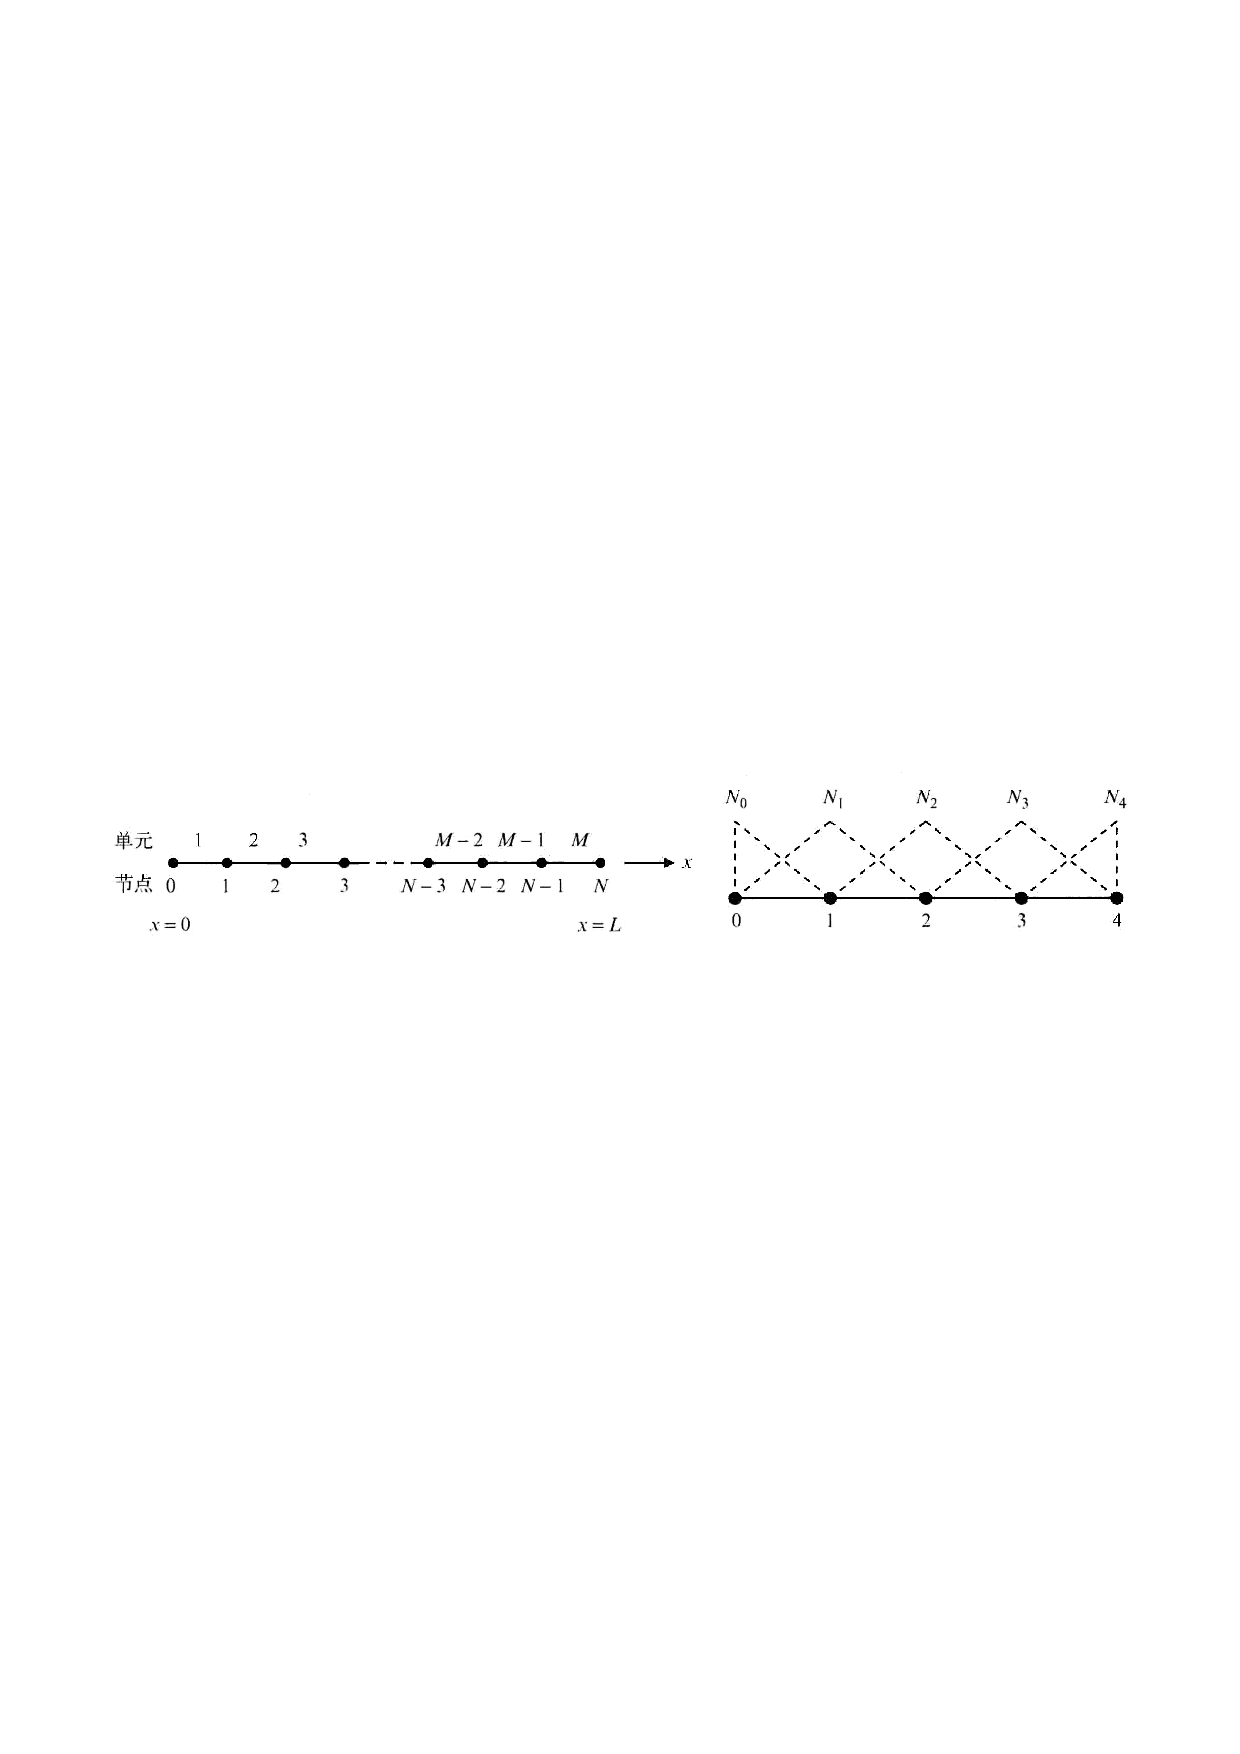
\includegraphics[scale=0.95]{3.1.2-1.pdf}
    \caption{一维网格和一维线性基函数}
    \label{一维网格和一维线性基函数}
\end{figure}

\par 有限元法的第一步是将求解区域 $(0,L)$ 划分成多个单元。
我们让单元
足够小,使得每个单元上的未知解可以通过对此单元两端节点上的值进行线性插值得到。
于是,未知解可表示为
\begin{equation}
    \varphi(x) = \sum_{j=0}^{N} \varphi_j N_j(x)
    =\sum_{j=1}^{N} \varphi_j N_j(x)
    +\varphi_0 N_0(x)
    =\sum_{j=1}^{N} \varphi_j N_j(x)
    +p N_0(x)
    \label{一维基函数展开}
\end{equation}
\par 其中 $\varphi_j$ 为未知量在第 $j$ 个节点处的值,
$N_j(x)$ 为相应的基函数。
$N_j(x)$ 是一个三角形函数,仅在第 $j$ 个单元与第 $j+1$ 个单
元上具有非零值。

\begin{theorem}{Galerkin 法}{一维算例 Galerkin 法}
    对于该一维 Helmholtz 方程,我们可以得到如下方程组
    \begin{equation}
        \sum_{j=1}^{N} K_{ij} \varphi_j = b_i \qquad i = 1, 2, \cdots, N
    \end{equation}
    其中
    \begin{align}
        K_{ij} &= 
        \int_{0}^{L}\left[
            \frac{\text{d}N_i(x)}{\text{d}x}\frac{\text{d}N_j(x)}{\text{d}x}
            - k^2N_i(x)N_j(x)
        \right]\text{d}x+\gamma\delta_{iN}\delta_{jN}\\
        b_i &= 
        -\int_{0}^{L}N_i(x)f(x)\text{d}x
        -p\int_{0}^{L}\left[
            \frac{\text{d}N_i(x)}{\text{d}x}\frac{\text{d}N_0(x)}{\text{d}x}
            - k^2N_i(x)N_0(x)
        \right]\text{d}x+q\delta_{iN}
    \end{align}
\end{theorem}

\begin{exercise}
    推导上述方程组。
\end{exercise}

\begin{solution}
    由 Galerkin 法,我们有
    \begin{equation*}
        \int_{0}^{L}N_i(x)\left[
            \frac{\text{d}^2\varphi(x)}{\text{d}x^2}+k^2\varphi(x)
        \right]\text{d}x = 
        \int_{0}^{L}N_i(x)f(x)\text{d}x
    \end{equation*}
    使用分部积分,得到
    \begin{gather*}
        \int_{0}^{L}N_i(x)
        \text{d}\left(\frac{\text{d}\varphi(x)}{\text{d}x}\right) 
        +\int_{0}^{L}
            k^2N_i(x)\varphi(x)
        \text{d}x = 
        \int_{0}^{L}N_i(x)f(x)\text{d}x\\
        \left.\left(
            N_i(x)\frac{\text{d}\varphi(x)}{\text{d}x}
        \right)\right|_0^L
        -\int_{0}^{L}
        \frac{\text{d}N_i(x)}{\text{d}x}
        \frac{\text{d}\varphi(x)}{\text{d}x}
        \text{d}x
        +\int_{0}^{L}
            k^2N_i(x)\varphi(x)
        \text{d}x = 
        \int_{0}^{L}N_i(x)f(x)\text{d}x\\
        \int_{0}^{L}\left[
            \frac{\text{d}N_i(x)}{\text{d}x}\frac{\text{d}\varphi(x)}{\text{d}x}
            - k^2N_i(x)\varphi(x)
        \right]\text{d}x
        -\left[N_i(x)\frac{\text{d}\varphi(x)}{\text{d}x}\right]_{x=L} = 
        -\int_{0}^{L}N_i(x)f(x)\text{d}x
    \end{gather*}
    将式 (\ref{一维边界条件-2}) 代入上式,得到
    \begin{equation*}
        \int_{0}^{L}\left[
            \frac{\text{d}N_i(x)}{\text{d}x}\frac{\text{d}\varphi(x)}{\text{d}x}
            - k^2N_i(x)\varphi(x)
        \right]\text{d}x
        -\left[N_i(L)\Big(q-\gamma\varphi(L)\Big)\right]= 
        -\int_{0}^{L}N_i(x)f(x)\text{d}x
    \end{equation*}
    将式 (\ref{一维基函数展开}) 代入,整理可得方程组
\end{solution}

\begin{note}
    只有当 $j=i\pm1$ 时,
    $N_i(x)$ 和 $N_j(x)$ 才会重叠,
    因此 $K_{ij}$ 中只有 $K_{ii}$、$K_{i+1,i}$ 
    和 $K_{i,i+1}$ 是非零的。
\end{note}

\begin{theorem}
    定理 \ref{thm:一维算例 Galerkin 法} 中的 $K_{ij}$
    可以直接计算得到解析式
    \begin{align}
        K_{ii}&=
        \left[
            \frac{1}{l^{(i)}}+\frac{1}{l^{(i+1)}}    
        \right]
        -k^2\left[
            \frac{l^{(i)}}{3}+\frac{l^{(i+1)}}{3}
        \right]
        \qquad i=1,2,\cdots,N-1\\
        K_{i+1,i}&=K_{i,i+1}=
        -\frac{1}{l^{(i)}}-k^2\frac{l^{(i)}}{6}
        \qquad i=1,2,\cdots,N-1\\
        K_{NN}&=\frac{1}{l^{(N)}}-k^2\frac{l^{(N)}}{3}
        +\gamma
    \end{align}
    其中,$l^{(i)}=x_{i+1}-x_i$ 为第 $i$ 个单元的长度。
    若源函数 $f(x)$ 在每个单元中可以近似为常数,则
    $b_i$ 也可以用解析方法求出
    \begin{align}
        b_1&=-f^{(1)}\frac{l^{(1)}}{2}
        -f^{(2)}\frac{l^{(2)}}{2}
        +\left(
            \frac{1}{l^{(1)}}+k^2\frac{l^{(1)}}{6}
        \right)p\\
        b_i&=-f^{(i)}\frac{l^{(i)}}{2}
        -f^{(i+1)}\frac{l^{(i+1)}}{2}\qquad i=2,3,\cdots,N-1\\
        b_N&=-f^{(N)}\frac{l^{(N)}}{2}+q
    \end{align}
    其中,$f^{(i)}$ 为源函数 $f(x)$ 在第 $i$ 个单元的平均值。
\end{theorem}

\par 与有限差分法类似,用有限元法模拟波的传播时,由于数值离散化,模拟波的波数将与
精确值略有不同。假设有一个均匀离散网格使得 $l^{(i)}=h$,考虑沿 $x$ 方向传播的平面波
\begin{equation}
    \varphi(x) = \varphi_0e^{-jkx}
\end{equation}
\par 此平面波的有限元解具有以下形式
\begin{equation}
    \varphi_i = \varphi_0e^{-j\tilde{k}ih}
    \label{一维有限元解}
\end{equation}

\begin{theorem}{一维数值色散}
    定理 \ref{thm:一维算例 Galerkin 法} 中给出公式的数值相位误差为
    \begin{equation}
        \frac{\tilde{k}-k}{k}
        \approx\frac{1}{12}(kh)^2
        =\frac{\pi^2}{3}\left(\frac{h}{\lambda}\right)^2
    \end{equation}
\end{theorem}

\begin{exercise}
    证明上述定理。
\end{exercise}

\begin{solution}
    将式 (\ref{一维有限元解}) 代入无源项的有限元方程中,得到
    \begin{gather*}
        K_{i,i-1}\varphi_{i-1}+K_{ii}\varphi_i+K_{i,i+1}\varphi_{i+1}
        =0\\
        -\left(\frac{1}{h}+k^2\frac{h}{6}\right)
        \varphi_{i-1}
        +2\left(\frac{1}{h}+-k^2\frac{h}{3}\right)
        \varphi_i
        -\left(\frac{1}{h}+k^2\frac{h}{6}\right)
        \varphi_{i+1}
        =0\\
        \left[
            -\left(\frac{1}{h}+k^2\frac{h}{6}\right)
            e^{j\tilde{k}h}
            +2\left(\frac{1}{h}-k^2\frac{h}{3}\right)
            -\left(\frac{1}{h}+k^2\frac{h}{6}\right)
            e^{-j\tilde{k}h}
        \right]\varphi_0e^{-j\tilde{k}ih}
        =0
    \end{gather*}
    整理得
    \begin{equation*}
        \left(
            \frac{1}{h}+k^2\frac{h}{6}
        \right)\cos(\tilde{k}h)
        =\frac{1}{h}-k^2\frac{h}{3}
    \end{equation*}
    解得数值波数的精确解为
    \begin{equation*}
        \tilde{k}=\frac{1}{h}
        \arccos\left(
            \frac{6-2(kh)^2}{6+(kh)^2}
        \right)
    \end{equation*}
    为了得到更明确的表达式,可把余弦函
    数用级数展开式的前两项近似表示,得到
    \begin{gather*}
        \left(
            \frac{1}{h}+k^2\frac{h}{6}
        \right)\left(
            1-\frac{(\tilde{k}h)^2}{2}
        \right)
        \approx\frac{1}{h}-k^2\frac{h}{3}\\
        \frac{\tilde{k}-k}{k}
        \approx\frac{1}{12}(kh)^2
        =\frac{\pi^2}{3}\left(\frac{h}{\lambda}\right)^2
    \end{gather*}
\end{solution}

\section{标量场的有限元分析}

\par 本节介绍二维或三维标量问题的有限元分析。

\subsection{边值问题}

\par 考虑求解区域 $\Omega$ 中由密度为 $\varrho_e$ 的电荷
产生的静电势 $\varphi$ 的问题。 
该区域可以是二维或三
维的,所填充介质的介电常数为 $\epsilon$。
基于 Maxwell 方程,电荷产生的电场满足下面两个方程:
\begin{align}
    \label{Maxwell 方程-1}
    \nabla\times\vec{E}&=0\\
    \label{Maxwell 方程-2}
    \nabla\cdot(\epsilon \vec{E})&=\varrho_e
\end{align}

\par 由矢量恒等式 $\nabla\times\nabla \varphi\equiv 0$ 可知,满足第一个方程的电场可表示为
\begin{equation}
    \vec{E}=-\nabla\varphi
    \label{电场与电势关系}
\end{equation}
\par 将式 (\ref{电场与电势关系}) 代入式 (\ref{Maxwell 方程-2}) 中,得到泊松方程
\begin{equation}
    -\nabla\cdot(\epsilon\nabla\varphi)=\varrho_e
    \qquad \text{在}\ \Omega\ \text{中}
    \label{泊松方程}
\end{equation}
\par 下面将边界条件假设为
\begin{align}
    \label{标量场边界条件-1}
    \varphi=\varphi_D\qquad \text{在}\ \Gamma_D\ \text{上}\\
    \label{标量场边界条件-2}
    \vec{n}\cdot(\epsilon\nabla\varphi)=\kappa_N\qquad \text{在}\ \Gamma_N\ \text{上}
\end{align}
\par 其中,$\varphi_D$ 为 Dirichlet 边界 
$\Gamma_D$ 上的电势的指定值,$\kappa_N$ 
为 Neumann 边界 $\Gamma_N$ 上的电势的法向
导数值。而 $\Gamma_D$ 和 $\Gamma_N$ 构成了
区域 $\Omega$ 的完整边界,记为 $\Gamma$。

\subsection{有限元公式的建立}

\par 常用的子域有二维中的三
角形单元和三维中的四面体单元。
当区域 $\Omega$ 被划分成小单元后,每个单元中的电势可以用诸
如线性、二次和三次函数的简单函数近似。
这种近似可以通过
对单元内一组离散点处的电势值进行插值得到。

\begin{theorem}
    三角形单元中的电势可以近似为
    \begin{equation}
        \varphi^e(x,y)=N_1^e(x,y)\varphi_1^e
        +N_2^e(x,y)\varphi_2^e
        +N_3^e(x,y)\varphi_3^e
    \end{equation}
    其中,$N_l^e(x,y)(l=1,2,3)$ 为插值函数,
    $\varphi_l^e(l=1,2,3)$ 为该单元中节点 $l$ 处的电势值。
    \begin{equation}
        N_l^e(x,y)=\frac{1}{2\Delta^e}
        (a_l^e+ b_l^ex+c_l^ey)
    \end{equation}
    其中
    \begin{equation}
        \Delta^e=\frac{1}{2}
        (b_1^ec_2^e-b_2^ec_1^e)
        =\ \text{单元}\ e\ \text{的面积}
    \end{equation}
    以及
    \begin{equation}
        \begin{gathered}
            a_1^e=x_2^ey_3^e-x_3^ey_2^e
            \qquad b_1^e=y_2^e-y_3^e
            \qquad c_1^e=x_3^e-x_2^e\\
            a_2^e=x_3^ey_1^e-x_1^ey_3^e
            \qquad b_2^e=y_3^e-y_1^e
            \qquad c_2^e=x_1^e-x_3^e\\
            a_3^e=x_1^ey_2^e-x_2^ey_1^e
            \qquad b_3^e=y_1^e-y_2^e
            \qquad c_3^e=x_2^e-x_1^e
        \end{gathered}
    \end{equation}
    其中,$(x_l^e,y_l^e)(l=1,2,3)$ 表示单元 $e$ 中节点 $l$ 的坐标。
\end{theorem}

\begin{exercise}
    推导上述定理。
\end{exercise}

\begin{solution}
    三角形单元中的电势可以近似为
    \begin{equation*}
        \varphi^e(x,y)=a+bx+cy
    \end{equation*}
    式中,上标 $e$ 表示该表达式限定在该特定单元上。将
    三角形单元的三个顶点代入上式,得到
    \begin{gather*}
        \varphi_1^e=a+bx_1^e+cy_1^e\\
        \varphi_2^e=a+bx_2^e+cy_2^e\\
        \varphi_3^e=a+bx_3^e+cy_3^e
    \end{gather*}
    解得 $a$、$b$ 和 $c$ 的值,代入整理得证。
\end{solution}

\begin{theorem}
    推导的插值函数具有以下特性
    \begin{equation}
        N_l^e(x^e_k,y^e_k)
        =\left\{
            \begin{aligned}
                &1\qquad l=k\\
                &0\qquad l\neq k
            \end{aligned}
        \right.
    \end{equation}
    该性质由插值函数在插值点处的值等于函数值易知。
\end{theorem}

\par 每个单元的电势值可以由节点处的值进行插值求得,
整个区域中的电势可表示为
\begin{equation}
    \varphi(x,y)=\sum_{j=1}^{N} \varphi_j N_j(x,y)
    +\sum_{j=1}^{N_D} \varphi_{j}^D N_{j}^D(x,y)
\end{equation}
\par 其中,$N$ 为电势值未知的节点总数,$N_D$ 为边界
$\Gamma_D$ 上的节点数。此
外,$\varphi_j$ 为节点 $j$ 处的电势,$N_j$ 为相应的插值函数
或基函数;$\varphi_j^D$和 $N_j^D$ 为 $\Gamma_D$ 上各节点相应的电势
值和插值函数。

\begin{note}
    $N_j$ 和 $N_j^D$ 由与相应节点直接相关
    的各单元内的插值函数构成。也就是说,
    $N_j$ 和 $N_j^D$ 由所有包含节点 $j$ 的插值函数 $N_l^e(x,y)$ 相加构成。
\end{note}

\begin{theorem}{弱式表达式}
    式 (\ref{泊松方程}),式 (\ref{标量场边界条件-1}) 和式
    (\ref{标量场边界条件-2}) 所定义的边值问题的弱式表达式为
    \begin{equation}
        \int_{\Omega}\epsilon\nabla w_i\cdot\nabla \varphi\text{d}\Omega
        =\int_{\Omega}w_i\varrho_e\text{d}\Omega
        +\int_{\Gamma_D}\vec{n}\cdot(\epsilon\nabla\varphi)w_i\text{d}\Gamma
        +\int_{\Gamma_N}\kappa_N w_i\text{d}\Gamma
    \end{equation}
\end{theorem}

\begin{exercise}
    证明上述定理。
\end{exercise}

\begin{solution}
    式 (\ref{泊松方程}) 两边乘以权函数 $w_i$ 并在整个求解区域 $\Omega$ 上积分,
    得到
    \begin{equation*}
        -\int_{\Omega}w_i[\nabla\cdot(\epsilon\nabla\varphi)]\text{d}\Omega
        = \int_{\Omega}w_i\varrho_e\text{d}\Omega
    \end{equation*}
    使用矢量恒等式
    \begin{equation*}
        w_i[\nabla\cdot(\epsilon\nabla\varphi)]
        =\nabla\cdot(w_i\epsilon\nabla\varphi)
        -\epsilon\nabla\varphi\cdot\nabla w_i
    \end{equation*}
    将其代入上式,得到
    \begin{gather*}
        \int_{\Omega}\epsilon\nabla w_i\cdot\nabla \varphi\text{d}\Omega
        =\int_{\Omega}w_i\varrho_e\text{d}\Omega
        +\int_{\Omega}\nabla\cdot(w_i\epsilon\nabla\varphi)\text{d}\Gamma\\
        \int_{\Omega}\epsilon\nabla w_i\cdot\nabla \varphi\text{d}\Omega
        =\int_{\Omega}w_i\varrho_e\text{d}\Omega
        +\int_{\Gamma}\vec{n}\cdot(w_i\epsilon\nabla\varphi)\text{d}\Gamma
    \end{gather*}
    将边界条件代入,得到
    \begin{equation*}
        \int_{\Omega}\epsilon\nabla w_i\cdot\nabla \varphi\text{d}\Omega
        =\int_{\Omega}w_i\varrho_e\text{d}\Omega
        +\int_{\Gamma_D}\vec{n}\cdot(\epsilon\nabla\varphi)w_i\text{d}\Gamma
        +\int_{\Gamma_N}\kappa_N w_i\text{d}\Gamma
    \end{equation*}
\end{solution}

\begin{theorem}{Galerkin 法}
    对于该边值问题,我们可以得到如下方程组
    \begin{equation}
        \sum_{j=1}^{N} K_{ij} \varphi_j = b_i \qquad i = 1, 2, \cdots, N
    \end{equation}
    其中
    \begin{align}
        \label{标量场有限元公式-1}
        K_{ij} &= 
        \int_{\Omega}\epsilon\nabla N_i\cdot\nabla N_j\text{d}\Omega \\
        \label{标量场有限元公式-2}
        b_i &= 
        \int_{\Omega}\varrho_e N_i\text{d}\Omega
        +\int_{\Gamma_N}\kappa_N N_i\text{d}\Gamma
        -\sum_{j=1}^{N_D}\varphi^D_j\int_{\Gamma}\epsilon\nabla N_i
        \cdot\nabla N_j^D\text{d}\Omega
    \end{align}
\end{theorem}

\par 在上面有限元法分析过程中,
为了计算 $K_{ij}$,需要知道 $N_i$ 和 $N_j$。
通常 $N_i$ 和 $N_j$ 的显
式表达式很难得到,因为每个节点都可能与不同形状和不同数量的单元相连接。
为克服此困难,可以将式 (\ref{标量场有限元公式-1}) 重写为
\begin{equation}
    K_{ij} = 
    \sum_{e=1}^{M}
    \int_{\Omega^e}\epsilon\nabla N_i\cdot\nabla N_j\text{d}\Omega
\end{equation}
\par 式中,$\Omega^e$ 表示单元 $e$ 的区域;$M$ 为区域 $\Omega$ 中单元的总数。
逐个计算每个单元对矩阵 $[K]$ 的贡献,选择对应的值相加,以此减少计算量。

\section{矢量场的有限元分析}

\par 有限元方法可以推广到处理矢量场的问题。

\subsection{边值问题}

\par 在介电常数为 $\epsilon$、
磁导率为 $\mu$ 的区域 $\Omega$ 中,
考虑如何求解由电流密度 $\vec{J}_{\text{imp}}$ 产生的电场强
度 $\vec{E}$,求解域可以是二维或三维的。
为了求得 $\vec{E}$,我们需要求解服从给定边界条件的 Maxwell 方程组
\begin{align}
    \label{Maxwell 频域方程组-1}
    \nabla\times\vec{E}&=-j\omega\mu\vec{H}\\
    \label{Maxwell 频域方程组-2}
    \nabla\times\vec{H}&=j\omega\epsilon\vec{E}+\vec{J}_{\text{imp}}\\
    \label{Maxwell 频域方程组-3}
    \nabla\cdot(\epsilon\vec{E})&=-\frac{1}{j\omega}\nabla\cdot\vec{J}_{\text{imp}}\\
    \label{Maxwell 频域方程组-4}
    \nabla\cdot(\mu\vec{H})&=0
\end{align}
\par 消去 $\vec{H}$,得到波动方程
\begin{equation}
    \nabla\times\left(
        \frac{1}{\mu_r}\nabla\times\vec{E}
    \right)-k_0^2\epsilon_r\vec{E}
    =-jk_0Z_0\vec{J}_{\text{imp}}
    \qquad \text{在}\ \Omega\ \text{中}
    \label{矢量波动方程}
\end{equation}
\par 其中,
$\epsilon_r=\frac{\epsilon}{\epsilon_0}$ 为相对介电常数,
$\mu_r=\frac{\mu}{\mu_0}$ 为相对磁导率,
$k_0=\omega\sqrt{\mu_0\epsilon_0}$ 为自由空间中的波数,
$Z_0=\sqrt{\frac{\mu_0}{\epsilon_0}}$ 为自由空间的特征阻抗。

\par 下面将边界条件假设为
\begin{align}
    \label{矢量场边界条件-1}
    \vec{n}\times\vec{E}&=\vec{P}
    \ \ \ \qquad \text{在}\ \Gamma_D\ \text{上}\\
    \label{矢量场边界条件-2}
    \vec{n}\times\left(
        \frac{1}{\mu_r}\nabla\times\vec{E}
    \right)
    +\frac{jk_0}{\eta_r}
    \vec{n}\times(\vec{n}\times\vec{E})
    &=\vec{K}_N
    \qquad \text{在}\ \Gamma_N\ \text{上}
\end{align}
\par 其中,$\vec{P}$为边界 $\Gamma_D$ 上的切向电场
值,$\eta_r$ 为 $\Gamma_N$ 上的归一化表面阻抗,
$\vec{K}_N$ 为已知函数,表示
边界 $\Gamma_N$ 上的边界源。

\subsection{有限元公式的建立}

\par 首先推导矢量场的插值函数。

\begin{theorem}
    三角形单元中的场可以用下面的公式进行插值
    \begin{equation}
        \vec{E}^e(x,y)=\vec{N}_{12}^e(x,y)E_{12}^e
        +\vec{N}_{13}^e(x,y)E_{13}^e
        +\vec{N}_{23}^e(x,y)E_{23}^e
        \label{矢量场插值函数}
    \end{equation}
    其中,$E_{lk}^e$ 表示单元 $e$ 中连接节点 $l$ 和 $k$ 的棱边上的
    电场切向分量,$\vec{N}_{lk}^e$ 表示相应的插值函数。
    
    若把三角形中与节点 $l$ 和 $k$ 相关的线性标量基函数
    分别表示为 $N_l^e$ 和 $N_k^e$,
    则式 (\ref{矢量场插值函数}) 中的矢量基函数可以写成
    \begin{equation}
        \vec{N}_{lk}^e
        =(N_l^e\nabla N_k^e-N_k^e\nabla N_l^e)\ell_{lk}^e
    \end{equation}
    其中,$\ell_{lk}^e$ 为连接节点 $l$ 和 $k$ 的带符号的边长。
\end{theorem}

\par 每一个单元中的电场 $\vec{E}$ 都可以用该
单元中棱边上的切向场分量值进行插值,所以
整个区域 $\Omega$ 中的电场 $\vec{E}$ 可以表示为
\begin{equation}
    \vec{E}=\sum_{j=1}^{N_{\text{edge}}}  E_j \vec{N}_j
    +\sum_{j=1}^{N_D} E_j^D \vec{N}_j^D
\end{equation}
\par 其中,$N_{\text{edge}}$ 为除了 $\Gamma_D$ 上的棱边的所有棱边总数,
$E_j$ 为第 $j$ 条棱边上 $\vec{E}$ 的切向分量,
$\vec{N}_j$ 为相应的矢量基函数。
此外,$N_D$ 为边界 $\Gamma_D$ 上的节点数,
$E_j^D$ 和 $\vec{N}_j^D$ 为这些棱边上的切向电场和相应的基函数。

\begin{theorem}{弱式表达式}
    式 (\ref{矢量波动方程}),式 (\ref{矢量场边界条件-1}) 和式
    (\ref{矢量场边界条件-2}) 所定义的边值问题的弱式表达式为
    \begin{equation}
        \begin{gathered}
            \int_{\Omega}\left[
            \frac{1}{\mu_r}
            (\nabla\times\vec{W}_i)\cdot(\nabla\times\vec{E})
            -k_0^2\epsilon_r\vec{W}_i\cdot\vec{E}
        \right]\text{d}\Omega
        =\int_{\Gamma_D}\frac{1}{\mu_r}
        (\vec{n}\times\vec{W}_i)\cdot(\nabla\times\vec{E})\text{d}\Gamma\\
        -\int_{\Gamma_N}\left[
            \frac{jk_0}{\eta_r}
            (\vec{n}\times\vec{W}_i)
            \cdot(\vec{n}\times\vec{E})
            +\vec{W}_i\cdot\vec{K}_N
        \right]\text{d}\Gamma
        -jk_0Z_0\int_{\Omega}\vec{W}_i\cdot\vec{J}_{\text{imp}}\text{d}\Omega
        \end{gathered}
    \end{equation}
\end{theorem}

\begin{exercise}
    证明上述定理。
\end{exercise}

\begin{solution}
    式 (\ref{矢量波动方程}) 两边乘以权函数 $\vec{W}_i$ 并在整个求解区域 $\Omega$ 上积分,
    得到
    \begin{equation*}
        \int_{\Omega}\vec{W}_i\cdot\left[
            \nabla\times\left(
                \frac{1}{\mu_r}\nabla\times\vec{E}
            \right)-k_0^2\epsilon_r\vec{E}
        \right]\text{d}\Omega
        =-jk_0Z_0
        \int_{\Omega}\vec{W}_i\cdot \vec{J}_{\text{imp}}\text{d}\Omega
    \end{equation*}
    使用矢量恒等式
    \begin{equation*}
        \nabla\cdot\left[
            \vec{W}_i\times\left(
                \frac{1}{\mu_r}\nabla\times\vec{E}
            \right)
        \right]
        =\frac{1}{\mu_r}
        (\nabla\times\vec{W}_i)\cdot(\nabla\times\vec{E})
        -\vec{W}_i\cdot\left[
            \nabla\times\left(
            \frac{1}{\mu_r}\nabla\times\vec{E}
        \right)
        \right]
    \end{equation*}
    将其代入上式,得到
    \begin{gather*}
        \int_{\Omega}\left[
            \frac{1}{\mu_r}
            (\nabla\times\vec{W}_i)\cdot(\nabla\times\vec{E})
            -k_0^2\epsilon_r\vec{W}_i\cdot\vec{E}
        \right]\text{d}\Omega
        =\int_{\Omega}\nabla\cdot\left[
            \vec{W}_i\times\left(
                \frac{1}{\mu_r}\nabla\times\vec{E}
            \right)
        \right]\text{d}\Omega
        -jk_0Z_0\int_{\Omega}\vec{W}_i\cdot\vec{J}_{\text{imp}}\text{d}\Omega\\
        \int_{\Omega}\left[
            \frac{1}{\mu_r}
            (\nabla\times\vec{W}_i)\cdot(\nabla\times\vec{E})
            -k_0^2\epsilon_r\vec{W}_i\cdot\vec{E}
        \right]\text{d}\Omega
        =\int_{\Gamma}
            \vec{n}\cdot\left[
                \vec{W}_i\times\left(
                \frac{1}{\mu_r}\nabla\times\vec{E}
            \right)
            \right]
        \text{d}\Gamma
        -jk_0Z_0\int_{\Omega}\vec{W}_i\cdot\vec{J}_{\text{imp}}\text{d}\Omega
    \end{gather*}
    再使用矢量恒等式
    \begin{equation*}
        \vec{n}\cdot\left(
            \vec{W}_i\times\left(
                \frac{1}{\mu_r}\nabla\times\vec{E}
            \right)
        \right)
        =\frac{1}{\mu_r}
        (\vec{n}\times\vec{W}_i)\cdot(\nabla\times\vec{E})
        -\vec{W}_i\cdot\left[
            \vec{n}\times\left(
            \frac{1}{\mu_r}\nabla\times\vec{E}
        \right)
        \right]
    \end{equation*}
    得到
    \begin{gather*}
        \int_{\Omega}\left[
            \frac{1}{\mu_r}
            (\nabla\times\vec{W}_i)\cdot(\nabla\times\vec{E})
            -k_0^2\epsilon_r\vec{W}_i\cdot\vec{E}
        \right]\text{d}\Omega
        =\int_{\Gamma}
            \frac{1}{\mu_r}
            (\vec{n}\times\vec{W}_i)\cdot(\nabla\times\vec{E})\text{d}\Gamma\\
        -\int_{\Gamma}
            \vec{W}_i\cdot\left[
                \vec{n}\times\left(
                \frac{1}{\mu_r}\nabla\times\vec{E}
            \right)
            \right]
        \text{d}\Gamma
        -jk_0Z_0\int_{\Omega}\vec{W}_i\cdot\vec{J}_{\text{imp}}\text{d}\Omega
    \end{gather*}
\end{solution}

\begin{theorem}{Galerkin 法}
    对于该边值问题,我们可以得到如下方程组
    \begin{equation}
        \sum_{j=1}^{N_{\text{edge}}} K_{ij} E_j = b_i \qquad i = 1, 2, \cdots, N_{\text{edge}}
    \end{equation}
    其中
    \begin{align}
        \nonumber
        K_{ij} = 
        &\ \int_{\Omega}\left[
            \frac{1}{\mu_r}
            (\nabla \times \vec{N}_i) \cdot (\nabla \times \vec{N}_j)
            -k_0^2\epsilon_r\vec{N}_i\cdot\vec{N}_j
        \right]\text{d}\Omega\\
        &+jk_0\int_{\Gamma_N}\left[
            \frac{1}{\eta_r}
            (\vec{n}\times\vec{N}_i)\cdot(\vec{n}\times\vec{N}_j)
        \right]\text{d}\Gamma\\
        \nonumber
        b_i = 
        &-jk_0Z_0\int_{\Omega}\vec{N}_i\cdot
        \vec{J}_{\text{imp}}\text{d}\Omega
        -\int_{\Gamma_N}\vec{N}_i\cdot\vec{K}_N\text{d}\Gamma\\
        &-\sum_{j=1}^{N_D}E_j^D\int_{\Gamma}\left[
            \frac{1}{\mu_r}
            (\nabla\times\vec{N}_i)\cdot(\nabla\times\vec{N}_j^D)
            -k_0^2\epsilon_r\vec{N}_i\cdot\vec{N}_j^D
        \right]\text{d}\Gamma
    \end{align}
\end{theorem}

\section{时域有限元分析}

\subsection{边值问题}

\par Maxwell 方程组的前两个方程,在时域中为
\begin{align}
    \label{Maxwell 时域方程组-1}
    \nabla\times\vec{\mathscr{E}}(t)&=-\mu\frac{\partial\vec{\mathscr{H}}(t)}{\partial t}\\
    \label{Maxwell 时域方程组-2}
    \nabla\times\vec{\mathscr{H}}(t)
    &=\epsilon\frac{\partial\vec{\mathscr{E}}(t)}{\partial t}
    +\sigma\vec{\mathscr{E}}(t)
    +\vec{\mathscr{J}}_{\text{imp}}(t)
\end{align}
\par 其中,$\sigma$ 为电导率。相应的边界条件为
\begin{align}
    \label{时域边界条件-1}
    \vec{n}\times\vec{\mathscr{E}}(t)&=\vec{\mathscr{P}}(t)
    \ \ \qquad \text{在}\ \Gamma_D\ \text{上}\\
    \label{时域边界条件-2}
    \vec{n}\times\left[
        \frac{1}{\mu}\nabla\times\vec{\mathscr{E}}(t)
    \right]
    +Y \vec{n}\times\left[
        \vec{n}\times\frac{\partial \vec{\mathscr{E}}(t)}{\partial t}
    \right]
    &=\vec{\mathscr{K}}_N(t)
    \qquad \text{在}\ \Gamma_N\ \text{上}
\end{align}
\par 其中,$Y$ 为边界 $\Gamma_N$ 的表面导纳。
从式 (\ref{Maxwell 时域方程组-1}) 和式 (\ref{Maxwell 时域方程组-2}) 中消去 $\vec{\mathscr{H}}(t)$,
得到电场的矢量波动方程为
\begin{equation}
    \nabla\times\left[
        \frac{1}{\mu}\nabla\times\vec{\mathscr{E}}(t)
    \right]+\epsilon\frac{\partial^2\vec{\mathscr{E}}(t)}{\partial t^2}
    +\sigma\frac{\partial\vec{\mathscr{E}}(t)}{\partial t}
    =-\frac{\partial \vec{\mathscr{J}}_{\text{imp}}(t)}{\partial t}
    \label{时域矢量波动方程}
\end{equation}

\subsection{有限元公式的建立}

\par 首先把求解空间划分成许多小的有限元,然后将每个单元中的电场用矢
量基函数展开,如此可将电场表示成
\begin{equation}
    \vec{\mathscr{E}}(\vec{r},t)=
    \sum_{j=1}^{N_{\text{edge}}}\vec{N}_j(\vec{r})\mathscr{E}_j(t)
    +\sum_{j=1}^{N_D}\vec{N}_j^D(\vec{r})\mathscr{E}_j^D(t)
\end{equation}

\begin{theorem}{弱式表达式}
    式 (\ref{时域矢量波动方程}),式 (\ref{时域边界条件-1}) 和式
    (\ref{时域边界条件-2}) 所定义的边值问题的弱式表达式为
    \begin{equation}
        \begin{aligned}
            \int_{\Omega}&\left[
                \frac{1}{\mu}
                (\nabla\times\vec{W}_i)\cdot(\nabla\times\vec{\mathscr{E}})
                +\epsilon\vec{W}_i\cdot\frac{\partial^2\vec{\mathscr{E}}}{\partial t^2}
                +\sigma\vec{W}_i\cdot\frac{\partial\vec{\mathscr{E}}}{\partial t}
            \right]\text{d}\Omega\\
            &=
            -\int_{\Gamma_N}\left[
                Y(\vec{n}\times\vec{W}_i)\cdot
                \left(
                    \vec{n}\times\frac{\partial\vec{\mathscr{E}}}{\partial t}
                \right)
                +\vec{W}_i\cdot\vec{\mathscr{K}}_N
            \right]\text{d}\Gamma
            -\int_{\Omega}\vec{W}_i\cdot
            \frac{\partial\vec{\mathscr{J}}_{\text{imp}}}{\partial t}\text{d}\Omega
        \end{aligned}
    \end{equation}
\end{theorem}

\begin{theorem}{Galerkin 法}{时域有限元方程}
    对于该边值问题,我们可以得到如下方程组
    \begin{equation}
        [T]\frac{\text{d}^2 \{\mathscr{E}\}}{\text{d}t^2}
        +[R]\frac{\text{d} \{\mathscr{E}\}}{\text{d}t}
        +[S]\{\mathscr{E}\}
        =\{\mathscr{f}\}
    \end{equation}
    其中
    \begin{align}
        T_{ij}&=
        \int_{\Omega}\epsilon\vec{N}_i\cdot\vec{N}_j\text{d}\Omega\\
        R_{ij}&=
        \int_{\Omega}\sigma\vec{N}_i\cdot\vec{N}_j\text{d}\Omega
        +\int_{\Gamma_N}Y(\vec{n}\times\vec{N}_i)\cdot
        (\vec{n}\times\vec{N}_j)\text{d}\Gamma\\
        S_{ij}&=
        \int_{\Omega}\frac{1}{\mu}
        (\nabla\times\vec{N}_i)\cdot(\nabla\times\vec{N}_j)\text{d}\Omega
    \end{align}
    另外,$\{\mathscr{E}\}=\left[\mathscr{E}_1,\mathscr{E}_2,
    \cdots,\mathscr{E}_{N_{\text{edge}}}\right]^T$,
    场源向量 $\{\mathscr{f}\}$ 的元素为
    \begin{equation}
        \begin{aligned}
            \mathscr{f}_i=
            &-\int_{\Omega}\vec{N}_i\cdot
            \frac{\partial\vec{\mathscr{J}}_{\text{imp}}}{\partial t}\text{d}\Omega
            -\int_{\Gamma_N}\vec{W}_i\cdot\vec{\mathscr{K}}_N\text{d}\Gamma\\
            &-\sum_{j=1}^{N_D}
            \int_{\Omega}\left[
                \frac{1}{\mu}
                (\nabla\times\vec{N}_i)\cdot(\nabla\times\vec{N}_j^D)\mathscr{E}_j^D
                +\vec{N}_i\cdot\vec{N}_j^D
                \left(
                    \epsilon\frac{\partial^2\mathscr{E}_j^D}{\partial t^2}
                    +\sigma\frac{\partial\mathscr{E}_j^D}{\partial t}
                \right)
            \right]\text{d}\Omega
        \end{aligned}
    \end{equation}    
\end{theorem}

\begin{theorem}{时间步进公式}
    在定理 \ref{thm:时域有限元方程} 中,对时间的一阶和二阶导数使用中心差分,得到
    时间步进公式
    \begin{equation}
        \begin{gathered}
            \left\{
                \frac{1}{(\Delta t)^2}[T]
                +\frac{1}{2\Delta t}[R]
            \right\}\{\mathscr{E}\}^{n+1}
            =\left\{
                \frac{2}{(\Delta t)^2}[T]
                -[S]
            \right\}\{\mathscr{E}\}^n\\
            -\left\{
                \frac{1}{(\Delta t)^2}[T]
                -\frac{1}{2\Delta t}[R]
            \right\}\{\mathscr{E}\}^{n-1}
            +\{\mathscr{f}\}^n
        \end{gathered}
    \end{equation}
    该公式具有二阶精度,以及有条件稳定。
\end{theorem}

\begin{theorem}{Newmark-beta 方法}
    从 Newmark-beta 积分法中推导的差分公式为
    \begin{align}
        \Big.\{\mathscr{E}\}\Big|_{t=n\Delta t}
        &\approx \beta\{\mathscr{E}\}^{n+1}
        +(1-2\beta)\{\mathscr{E}\}^{n}
        +\beta\{\mathscr{E}\}^{n-1}\\
        \Big.\{\mathscr{f}\}\Big|_{t=n\Delta t}
        &\approx \beta\{\mathscr{f}\}^{n+1}
        +(1-2\beta)\{\mathscr{f}\}^{n}
        +\beta\{\mathscr{f}\}^{n-1}
    \end{align}
\end{theorem}

\begin{theorem}{时间步进公式}
    使用从 Newmark-beta 方法推导的时间步进公式
    \begin{equation}
        \begin{aligned}
            &\left\{
                \frac{1}{(\Delta t)^2}[T]
                +\frac{1}{2\Delta t}[R]
                +\beta [S]
            \right\}\{\mathscr{E}\}^{n+1}
            =\left\{
                \frac{2}{(\Delta t)^2}[T]
                -(1-2\beta)[S]
            \right\}\{\mathscr{E}\}^n\\
            &\quad-\left\{
                \frac{1}{(\Delta t)^2}[T]
                -\frac{1}{2\Delta t}[R]
                +\beta [S]
            \right\}\{\mathscr{E}\}^{n-1}
            +\beta\{\mathscr{f}\}^{n+1}
            +(1-2\beta)\{\mathscr{f}\}^{n}
            +\beta\{\mathscr{f}\}^n
        \end{aligned}
    \end{equation}
    该公式具有二阶精度,当 $\beta\geq\frac{1}{4}$ 时无条件稳定。
\end{theorem}

\section{时域间断 Galerkin 法}

\subsection{时域间断 Galerkin 法的基本思想}

\par 考虑一个简单的一维波动方程
\begin{equation}
    \frac{1}{c}\frac{\partial \varphi(x,t)}{\partial t}
    -\frac{\partial \varphi(x,t)}{\partial x}=0
    \label{一维时域波动方程}
\end{equation}
\par 首先将该区域 $(0,L)$ 分成小的单元。
然后将式 (\ref{一维时域波动方程}) 乘以一个测试函数 $w^e$,
并且在单元 $e$ 上积分,得到
\begin{equation}
    \int_{x_1^e}^{x_2^e}w^e\left[
        \frac{1}{c}\frac{\partial \varphi}{\partial t}
        -\frac{\partial \varphi}{\partial x}
    \right]\text{d}x=0
\end{equation}
\par 其中,$x_1^e$ 与 $x_2^e$ 表示单元 $e$ 的两个端点。
使用分部积分法,可以得到弱式表达式
\begin{equation}
    \int_{x_1^e}^{x_2^e}\left[
        w^e\frac{1}{c}\frac{\partial \varphi}{\partial t}
        +\varphi\frac{\partial w^e}{\partial x}
    \right]\text{d}x
    =\Big.(\varphi w^e)\Big|_{x_1^e}^{x_2^e}
    \label{一维时域波动方程弱式}
\end{equation}

\begin{definition}{数值通量}
    为了使单元 $e$ 与其相邻单元耦合,引入数值通量的概念,
    记为 $\text{f}$。
    一种选择为中心通量
    \begin{equation}
        \text{f}=\frac{1}{2}(\varphi+\varphi^+)
    \end{equation}
    另一种选择为中心通量
    \begin{equation}
        \text{f}=\varphi^+
    \end{equation}
    其中,$\varphi^+$ 表示紧邻单元外侧的 $\varphi$ 值。

    这两种选择可以统一地写成
    \begin{equation}
        \text{f}=\frac{1}{2}(\varphi+\varphi^+)
        +\frac{1-\alpha}{2}(\varphi^+-\varphi)
    \end{equation}
    当 $\alpha=1$ 时为中心通量;当 $\alpha=0$ 时为迎风通量。
\end{definition}

\par 用数值通量来代替
式 (\ref{一维时域波动方程弱式}) 右边的 $\varphi$,得到
\begin{equation}
    \int_{x_1^e}^{x_2^e}\left[
        w^e\frac{1}{c}\frac{\partial \varphi}{\partial t}
        +\varphi\frac{\partial w^e}{\partial x}
    \right]\text{d}x
    =\Big.(\text{f} w^e)\Big|_{x_1^e}^{x_2^e}
\end{equation}
\par 从弱式表达式出发,再应用一次分部积分,可以反推得到强式表达式
\begin{equation}
    \int_{x_1^e}^{x_2^e}w^e\left[
        \frac{1}{c}\frac{\partial \varphi}{\partial t}
        -\frac{\partial \varphi}{\partial x}
    \right]\text{d}x
    =\Big.\big[(\text{f}-\varphi) w^e\big]\Big|_{x_1^e}^{x_2^e}
\end{equation}
\par 下面使用基函数 $N_j^e$ 把单元 $e$ 中的 $\varphi$ 展开为
\begin{equation}
    \varphi^e(x,t)=\sum_{j=1}^{N}N_j^e(x)\varphi_j(t)
\end{equation}
\par 其中,$p$ 为基函数的阶数。

\begin{theorem}
    对于该问题,我们可以得到如下方程组
    \begin{equation}
        [T^e]\frac{\text{d}\{\varphi^e\}}{\text{d}t}
        -[S^e]\{\varphi^e\}
        =\{\mathscr{f}^e\}
    \end{equation}
    其中
    \begin{align}
        T_{ij}^e&=
        \int_{x_1^e}^{x_2^e}
        \frac{1}{c}N_i^eN_j^e\text{d}x\\
        S_{ij}^e&=
        \int_{x_1^e}^{x_2^e}
        N_i^e\frac{\partial N_j^e}{\partial x}
        \text{d}x-\frac{2-\alpha}{2}
        \Big.(N_i^e N_j^e)\Big|_{x_1^e}^{x_2^e}\\
        \mathscr{f}_i^e&=
        \frac{2-\alpha}{2}\Big.(N_i^e\varphi^+)\Big|_{x_1^e}^{x_2^e}
    \end{align}
\end{theorem}

\subsection{中心通量时域间断 Galerkin 法}

\par 为了清晰起见,我们在建立公式时暂时忽略传导损耗项和源项。
首先使用矢量函数 $\vec{W}_i$ 测试式 (\ref{Maxwell 时域方程组-1}) 
和式 (\ref{Maxwell 时域方程组-2}) 给出的 Maxwell 方程,
并在一个单元内积分,得到
\begin{align}
    \int_{\Omega^e}\vec{W}_i\cdot\left(
        \epsilon\frac{\partial\vec{\mathscr{E}}}{\partial t}
        -\nabla\times\vec{\mathscr{H}}
    \right)\text{d}\Omega&=0\\
    \int_{\Omega^e}\vec{W}_i\cdot\left(
        \mu\frac{\partial\vec{\mathscr{H}}}{\partial t}
        +\nabla\times\vec{\mathscr{E}}
    \right)\text{d}\Omega&=0
\end{align}
\par 其中,$\Omega^e$ 表示第 $e$ 个单元的区域。
应用矢量恒等式
$\vec{W}_i\cdot(\nabla\times \vec{A})
=\nabla\cdot(\vec{A}\times\vec{W}_i)+\vec{A}\cdot(\nabla\times\vec{W}_i)$
和 Gauss 定理,得到弱式表达式
\begin{align}
    \int_{\Omega^e}\left[
        \epsilon\vec{W}_i\cdot\frac{\partial\vec{\mathscr{E}}}{\partial t}
        -(\nabla\times\vec{W}_i)\cdot\vec{\mathscr{H}}
    \right]\text{d}\Omega
    &=\oint_{\Gamma^e}\vec{W}_i\cdot(\vec{n}\times\vec{\mathscr{H}})\text{d}\Gamma\\
    \int_{\Omega^e}\left[
        \mu\vec{W}_i\cdot\frac{\partial\vec{\mathscr{H}}}{\partial t}
        +(\nabla\times\vec{W}_i)\cdot\vec{\mathscr{E}}
    \right]\text{d}\Omega
    &=-\oint_{\Gamma^e}\vec{W}_i\cdot(\vec{n}\times\vec{\mathscr{E}})\text{d}\Gamma
\end{align}
\par 其中,$\Gamma^e$ 表示包围 $\Omega^e$ 的边界。
为了将单元内部场与外部场 $(\mathscr{E}^+, \mathscr{H}^+)$ 耦合,将
$\vec{n}\times\mathscr{H}$ 用一个数值通量 $\mathscr{F}_{\text{h}}$ 替换,
将 $\vec{n}\times\mathscr{E}$ 用另一个数值通量 $\mathscr{F}_{\text{e}}$ 替换,
得到
\begin{align}
    \int_{\Omega^e}\left[
        \epsilon\vec{W}_i\cdot\frac{\partial\vec{\mathscr{E}}}{\partial t}
        -(\nabla\times\vec{W}_i)\cdot\vec{\mathscr{H}}
    \right]\text{d}\Omega
    &=\oint_{\Gamma^e}\vec{W}_i\cdot\mathscr{F}_{\text{h}}\text{d}\Gamma\\
    \int_{\Omega^e}\left[
        \mu\vec{W}_i\cdot\frac{\partial\vec{\mathscr{H}}}{\partial t}
        +(\nabla\times\vec{W}_i)\cdot\vec{\mathscr{E}}
    \right]\text{d}\Omega
    &=-\oint_{\Gamma^e}\vec{W}_i\cdot\mathscr{F}_{\text{e}}\text{d}\Gamma
\end{align}
\par 从弱式表达式出发,逆向应用矢量恒等式和 Gauss 定理,可以反推得到强式表达式
\begin{align}
    \label{时域间断 Galerkin 法强式表达式-1}
    \int_{\Omega^e}\vec{W}_i\cdot\left(
        \epsilon\frac{\partial\vec{\mathscr{E}}}{\partial t}
        -\nabla\times\vec{\mathscr{H}}
    \right)\text{d}\Omega
    &=\oint_{\Gamma^e}\vec{W}_i\cdot
    (\mathscr{F}_{\text{h}}-\vec{n}\times\vec{\mathscr{H}})\text{d}\Gamma\\
    \label{时域间断 Galerkin 法强式表达式-2}
    \int_{\Omega^e}\vec{W}_i\cdot\left(
        \mu\frac{\partial\vec{\mathscr{H}}}{\partial t}
        +\nabla\times\vec{\mathscr{E}}
    \right)\text{d}\Omega
    &=-\oint_{\Gamma^e}\vec{W}_i\cdot
    (\mathscr{F}_{\text{e}}-\vec{n}\times\vec{\mathscr{E}})\text{d}\Gamma
\end{align}
\par 使用中心通量
\begin{equation}
    \mathscr{F}_{\text{e}}=\frac{1}{2}
    \Big[\vec{n}\times(\mathscr{E}+\vec{\mathscr{E}}^+)\Big]
    \qquad
    \mathscr{F}_{\text{h}}=\frac{1}{2}
    \Big[\vec{n}\times(\mathscr{H}+\vec{\mathscr{H}}^+)\Big]
\end{equation}
\par 式 (\ref{时域间断 Galerkin 法强式表达式-1}) 和式 (\ref{时域间断 Galerkin 法强式表达式-2})
可以写成
\begin{align}
    \label{中心通量时域间断 Galerkin 法-1}
    \int_{\Omega^e}\vec{W}_i\cdot\left(
        \epsilon\frac{\partial\vec{\mathscr{E}}}{\partial t}
        -\nabla\times\vec{\mathscr{H}}
    \right)\text{d}\Omega
    &=\frac{1}{2}\oint_{\Gamma^e}\vec{W}_i\cdot
    \Big[\vec{n}\times(\mathscr{H}^+-\vec{\mathscr{H}})\Big]
    \text{d}\Gamma\\
    \label{中心通量时域间断 Galerkin 法-2}
    \int_{\Omega^e}\vec{W}_i\cdot\left(
        \mu\frac{\partial\vec{\mathscr{H}}}{\partial t}
        +\nabla\times\vec{\mathscr{E}}
    \right)\text{d}\Omega
    &=-\frac{1}{2}\oint_{\Gamma^e}\vec{W}_i\cdot
    \Big[\vec{n}\times(\mathscr{E}^+-\vec{\mathscr{E}})\Big]
    \text{d}\Gamma
\end{align}
\par 导电边界上的边界条件可以通过
两种方式实现:一种是直接规定边界上的未知数为零;
另一种是将场设置为以下形式
\begin{equation}
    \vec{n}\times\vec{\mathscr{E}}^+=
    -\vec{n}\times\vec{\mathscr{E}}
    \qquad
    \vec{n}\times\vec{\mathscr{H}}^+=
    -\vec{n}\times\vec{\mathscr{H}}
\end{equation}
\par 而混合边界条件,包括阻抗边界条件和一阶吸收边界条件,可以通过下面的设置来满足
\begin{equation}
    \vec{n}\times\vec{\mathscr{E}}^+=
    -Z_s\vec{n}\times
    (\vec{n}\times\vec{\mathscr{H}})
    \qquad
    \vec{n}\times\vec{\mathscr{H}}^+=
    Y_s\vec{n}\times
    (\vec{n}\times\vec{\mathscr{E}})
\end{equation}
\par 在这种情况下,式 (\ref{中心通量时域间断 Galerkin 法-1}) 和式 (\ref{中心通量时域间断 Galerkin 法-2})
可以写成
\begin{align}
    \int_{\Omega^e}\vec{W}_i\cdot\left(
        \epsilon\frac{\partial\vec{\mathscr{E}}}{\partial t}
        -\nabla\times\vec{\mathscr{H}}
    \right)\text{d}\Omega
    &=-\frac{1}{2}\oint_{\Gamma^e\cap\Gamma_M}
    \Big[
        Y_s(\vec{n}\times\vec{W}_i)\cdot
        (\vec{n}\times\vec{\mathscr{E}})
        +\vec{W}_i\cdot
        (\vec{n}\times\vec{\mathscr{H}})
    \Big]\text{d}\Gamma\\
    \int_{\Omega^e}\vec{W}_i\cdot\left(
        \mu\frac{\partial\vec{\mathscr{H}}}{\partial t}
        +\nabla\times\vec{\mathscr{E}}
    \right)\text{d}\Omega
    &=-\frac{1}{2}\oint_{\Gamma^e\cap\Gamma_M}
    \Big[
        Z_s(\vec{n}\times\vec{W}_i)\cdot
        (\vec{n}\times\vec{\mathscr{H}})
        -\vec{W}_i\cdot
        (\vec{n}\times\vec{\mathscr{E}})
    \Big]\text{d}\Gamma
\end{align}
\par 其中,$\Gamma_M$ 表示阻抗边界,
$\Gamma^e\cap\Gamma_M$ 表示 $\Gamma^e$ 中与阻抗边界相同的部分。

\begin{theorem}{Galerkin 法}{中心通量时域间断 Galerkin 法方程}
    对于该问题,我们可以得到如下方程组
    \begin{align}
        [T^e_{\text{e}}]\frac{\text{d}\{\mathscr{E}^e\}}{\text{d}t}
        -[S^e]\{\mathscr{H}^e\}
        &=\{\mathscr{f}^e_\text{e}\}
        -[R^e_{\text{e}}]\{\mathscr{E}^e\}
        +\{\mathscr{b}^e_\text{e}\}\\
        [T^e_{\text{h}}]\frac{\text{d}\{\mathscr{H}^e\}}{\text{d}t}
        +[S^e]\{\mathscr{E}^e\}
        &=\{\mathscr{f}^e_\text{h}\}
        -[R^e_{\text{h}}]\{\mathscr{H}^e\}
        +\{\mathscr{b}^e_\text{h}\}
    \end{align}
    其中
    \begin{align}
        T^e_{\text{e}}(i,j)&=
        \int_{\Omega^e}\epsilon\vec{N}_i^e\cdot\vec{N}_j^e\text{d}\Omega\\
        T^e_{\text{h}}(i,j)&=
        \int_{\Omega^e}\mu\vec{N}_i^e\cdot\vec{N}_j^e\text{d}\Omega\\
        S^e(i,j)&=
        \frac{1}{2}\int_{\Omega^e}
        \Big[
            \vec{N}_i^e\cdot(\nabla\times\vec{N}_j^e)
            +(\nabla\times\vec{N}_i^e)\cdot\vec{N}_j^e
        \Big]
        \text{d}\Omega\\
        R^e_{\text{e}}(i,j)&=
        \int_{\Omega^e}\sigma_{\text{e}}\vec{N}_i^e\cdot\vec{N}_j^e\text{d}\Gamma
        +\frac{1}{2}\int_{\Gamma^e\cap\Gamma_M}
        Y_s(\vec{n}\times\vec{N}_i^e)\cdot(\vec{n}\times\vec{N}_j^e)\text{d}\Gamma\\
        R^e_{\text{h}}(i,j)&=
        \int_{\Omega^e}\sigma_{\text{m}}\vec{N}_i^e\cdot\vec{N}_j^e\text{d}\Gamma
        +\frac{1}{2}\int_{\Gamma^e\cap\Gamma_M}
        Z_s(\vec{n}\times\vec{N}_i^e)\cdot(\vec{n}\times\vec{N}_j^e)\text{d}\Gamma\\
        \mathscr{f}^e_\text{e}(i)&=
        \frac{1}{2}\int_{\Gamma^e\cap\Gamma_I}
        \vec{N}_i^e\cdot(\vec{n}\times\vec{\mathscr{H}}^+)\text{d}\Gamma\\
        \mathscr{f}^e_\text{h}(i)&=
        \frac{1}{2}\int_{\Gamma^e\cap\Gamma_I}
        (\vec{n}\times\vec{N}_i^e)\cdot\mathscr{E}^+\text{d}\Gamma\\
        \mathscr{b}^e_\text{e}(i)&=
        -\int_{\Omega^e}\vec{N}_i^e\cdot
        \vec{\mathscr{J}}_{\text{imp}}\text{d}\Omega\\
        \mathscr{b}^e_\text{h}(i)&=
        -\int_{\Omega^e}\vec{N}_i^e\cdot
        \vec{\mathscr{M}}_{\text{imp}}\text{d}\Omega
    \end{align}
    其中,$\Gamma_I$ 表示单元之间的界面。
    需要注意,方程组中包含了传导损
    耗 $(\sigma_{\text{e}},\sigma_{\text{m}})$ 
    和外加源 $(\vec{\mathscr{J}}_{\text{imp}},
    \vec{\mathscr{M}}_{\text{imp}})$,以使这两个公式更具一般性。
\end{theorem}

\begin{theorem}{时间步进公式}
    在定理 \ref{thm:中心通量时域间断 Galerkin 法方程} 中,对时间的一阶导数使用中心差分,得到
    时间步进公式
    \begin{equation}
        \begin{aligned}
            \left(
                \frac{1}{\Delta t}[T^e_{\text{e}}]
                +\frac{1}{2}[R^e_{\text{e}}]
            \right)\{\mathscr{E}^e\}^{n+1}
            =&\left(
                \frac{1}{\Delta t}[T^e_{\text{e}}]
                -\frac{1}{2}[R^e_{\text{e}}]
            \right)\{\mathscr{E}^e\}^{n}
            +[S^e]\{\mathscr{H}^e\}^{n+\frac{1}{2}}\\
            &+\{\mathscr{f}^e_{\text{e}}\}^{n+\frac{1}{2}}
            +\{\mathscr{b}^e_{\text{e}}\}^{n+\frac{1}{2}}
        \end{aligned}
    \end{equation}
    \begin{equation}
        \begin{aligned}
            \left(
                \frac{1}{\Delta t}[T^e_{\text{h}}]
                +\frac{1}{2}[R^e_{\text{h}}]
            \right)\{\mathscr{H}^e\}^{n+\frac{3}{2}}
            =&\left(
                \frac{1}{\Delta t}[T^e_{\text{h}}]
                -\frac{1}{2}[R^e_{\text{h}}]
            \right)\{\mathscr{H}^e\}^{n+\frac{1}{2}}
            -[S^e]\{\mathscr{E}^e\}^{n+1}\\
            &+\{\mathscr{f}^e_{\text{h}}\}^{n+1}
            +\{\mathscr{b}^e_{\text{h}}\}^{n+1}
        \end{aligned}
    \end{equation}
    这两个公式可以用来以蛙跳的方式逐个单元、逐个时间步地计算电场和磁场,
    即 $\{\mathscr{E}^e\}^{n}
    \rightarrow \{\mathscr{H}^e\}^{n+\frac{1}{2}}
    \rightarrow \{\mathscr{E}^e\}^{n+1}
    \rightarrow \{\mathscr{H}^e\}^{n+\frac{3}{2}}$。
\end{theorem}

\subsection{迎风通量时域间断 Galerkin 法}

\section{吸收边界条件}

\subsection{二维吸收边界条件}

\par 在有限差分法中介绍过二维吸收边界条件。
但是那些条件都是针对平面边界推导
的,而在有限元法中可以使用曲面边界截断网格,
因此需要使用能充分考虑曲率影响的吸收边
界条件。

\begin{theorem}{一阶吸收边界条件}
    一阶吸收边界条件为
    \begin{equation}
        \frac{\partial \varphi}{\partial \rho}
        \approx
        \left(
            -jk-\frac{1}{2\rho}
        \right)\varphi
    \end{equation}
\end{theorem}

\begin{exercise}
    推导一阶吸收边界条件。
\end{exercise}

\begin{solution}
    曲面边界的吸收边界条件可以由波函数解的渐近形式推导得到。对于二维情况,远离
    源处的场可以表示为
    \begin{equation*}
        \varphi(\rho,\phi)=A(\phi)\frac{e^{-jk\rho}}{\sqrt{\rho}}
    \end{equation*}
    对 $\rho$ 求导,得到
    \begin{equation*}
        \frac{\partial \varphi}{\partial \rho}
        \approx
        \left(
            -jk-\frac{1}{2\rho}
        \right)A(\phi)\frac{e^{-jk\rho}}{\sqrt{\rho}}
        =
        \left(
            -jk-\frac{1}{2\rho}
        \right)\varphi
    \end{equation*}
\end{solution}

\begin{theorem}{二阶吸收边界条件}
    二阶吸收边界条件为
    \begin{equation}
        \frac{\partial \varphi}{\partial \rho}
        \approx
        \left(
            -jk-\frac{1}{2\rho}
            +\frac{1}{8jk\rho^2}
            +\frac{1}{8k^2\rho^3}
        \right)\varphi
        +\left(
            \frac{1}{2jk\rho^2}
            +\frac{1}{2k^2\rho^3}
        \right)\frac{\partial^2 \varphi}{\partial \phi^2}
    \end{equation}
\end{theorem}

\begin{exercise}
    推导二阶吸收边界条件。
\end{exercise}

\begin{solution}
    考虑使用下面更准确的渐近形式的波函数解
    \begin{equation*}
        \varphi(\rho,\phi)=
        \frac{e^{-jk\rho}}{\sqrt{\rho}}
        \sum_{n=0}^{\infty}\frac{a_n(\phi)}{\rho^n}
    \end{equation*}
    将上式代入极坐标形式的 Helmholtz 方程,即
    \begin{equation*}
        \frac{1}{\rho}\frac{\partial}{\partial \rho}
        \left(
            \rho\frac{\partial \varphi}{\partial \rho}
        \right)
        +\frac{1}{\rho^2}\frac{\partial^2 \varphi}{\partial \phi^2}
        +k^2\varphi=0
    \end{equation*}
    得到 $a_n(\phi)$ 的递推关系为
    \begin{equation*}
        -2jk(n+1)a_{n+1}=
        \left(n+\frac{1}{2}\right)^2
        a_n+\frac{\partial^2 a_n}{\partial \phi^2}
    \end{equation*}
    波函数解对 $\rho$ 求导,得到
    \begin{equation*}
        \frac{\partial \varphi}{\partial \rho}
        =\left(
            -jk-\frac{1}{2\rho}
        \right)\varphi
        -\frac{e^{-jk\rho}}{\sqrt{\rho}}
        \sum_{n=1}^{\infty}\frac{n a_n(\phi)}{\rho^{n+1}}
    \end{equation*}
    保留靠前的几项,经过一些处理之后得到
    \begin{equation*}
        \frac{\partial \varphi}{\partial \rho}
        =
        \left(
            -jk-\frac{1}{2\rho}
            +\frac{1}{8jk\rho^2}
            +\frac{1}{8k^2\rho^3}
        \right)\varphi
        +\left(
            \frac{1}{2jk\rho^2}
            +\frac{1}{2k^2\rho^3}
        \right)\frac{\partial^2 \varphi}{\partial \phi^2}
        +\mathcal{O}\left(\frac{1}{\rho^{\frac{9}{2}}}\right)
    \end{equation*}
\end{solution}

\par 保留靠前的更多项,上面描述的渐进方法可用于推导更高阶的吸收边界条件。

\begin{theorem}
    对于非圆形的边界,吸收边界条件可以通过下面的替换获得
    \begin{equation}
        \frac{\partial}{\partial \rho}
        \rightarrow
        \frac{\partial}{\partial n}
        \qquad
        \frac{1}{\rho}
        \rightarrow
        \kappa(s)
        \qquad
        \frac{1}{\rho^2}
        \frac{\partial^2}{\partial \phi^2}  
        \rightarrow
        \frac{\partial^2}{\partial s^2}
    \end{equation}
    其中,$s$ 表示沿边界度量的长度,$\kappa(s)$ 表示边界的曲率。

    一阶和二阶吸收边界条件变为
    \begin{align}
        \frac{\partial \varphi}{\partial n}
        &\approx
        \left(
            -jk-\frac{\kappa}{2}
        \right)\varphi\\
        \frac{\partial \varphi}{\partial n}
        &\approx
        \left(
            -jk-\frac{\kappa}{2}
            +\frac{\kappa^2}{8jk}
            +\frac{\kappa^3}{8k^2}
        \right)\varphi
        +\left(
            \frac{1}{2jk}
            +\frac{\kappa}{2k^2}
        \right)\frac{\partial^2 \varphi}{\partial s^2}
    \end{align}
\end{theorem}

\subsection{三维吸收边界条件}

\begin{theorem}{一阶吸收边界条件}
    对于三维电磁问题,最简单的吸收边界条件是 Sommerfeld 辐射条件,
    表示为
    \begin{equation}
        \vec{n}\times(\nabla\times\vec{E})
        \approx
        -jk\vec{n}\times(\vec{n}\times\vec{E})
    \end{equation}
    其中,$\vec{n}$ 为吸收表面的单位法向矢量。
\end{theorem}

\subsection{理想匹配层}
\chapter{矩量法}

\section{矩量法概述}

\par Maxwell 方程的解可以通过不同的方式得到。
除偏微分方程之外,也可以求解从 Maxwell 方程出发导出的积分
方程。

\par 例如,对于静电场问题,可以用 Green 函数法推导积分方程。
如果希望求解一块金属导体的电容,可以先建立一个积分方程来求解
导体表面的电荷。使用 Green 函数法,由线性叠加原理,可以写出
由金属导体表面电荷产生的总电势,即
\begin{equation}
    \varphi(\vec{r}) = 
    \iint_{S} G(\vec{r}, \vec{r}') \varrho_s(\vec{r}') \text{d}S'
    =\iint_{S} \frac{1}{4\pi\epsilon\left|\vec{r}-\vec{r}'\right|} 
    \varrho_s(\vec{r}') \text{d}S'
\end{equation}
\par 其中,$S$ 为金属体表面,
$\varrho_s(\vec{r}')$ 为金属表面的面电荷密度,
$\varphi(\vec{r})$ 为由面电荷产生的电势。
\par 在金属表面 $S$ 上,$\varphi(\vec{r})$
必须为常数,记为 $\Phi$,由此有
\begin{equation}
    \Phi = 
    \iint_{S} G(\vec{r}, \vec{r}') \varrho_s(\vec{r}') \text{d}S'
    \qquad
    \vec{r} \in S
    \label{金属表面积分方程}
\end{equation}
\par 上式就是一个积分方程,式中 $\Phi$ 为已知常数,
$G(\vec{r}, \vec{r}')$ 为已知函数,而 $\varrho_s(\vec{r}')$ 则为未知的金
属表面电荷密度,通过求解此积分方程可以得到 $\varrho_s(\vec{r}')$。
\par 为了使式 (\ref{金属表面积分方程}) 能使用计算机求解,可以用矩
量法在有限维子空间中对其解进行近似。首先,选择一组基函数用于
对 $\varrho_s(\vec{r}')$ 的近似,即
\begin{equation}
    \varrho_s(\vec{r}') = \sum_{j=1}^{N} c_j v_j(\vec{r}')
    \label{矩量法基函数展开}
\end{equation}
\par 其中,$v_j(\vec{r}')$ 为基函数,$c_j$ 为待定系数。
\par 选定基函数后,将式 (\ref{矩量法基函数展开}) 代人式 (\ref{金属表面积分方程}),
得到一个有限自由度的方程
\begin{equation}
    \sum_{j=1}^{N} c_j 
    \iint_{S} G(\vec{r}, \vec{r}') v_j(\vec{r}') \text{d}S'
    =\Phi
    \qquad
    \vec{r} \in S
    \label{矩量法方程}
\end{equation}
\par 为了求解 $c_j$,需要把上式转换为矩阵方程。
为此,选择一组函数 $w_1(\vec{r}),w_2(\vec{r}),\cdots,w_N(\vec{r})$,在
式 (\ref{矩量法方程}) 等号两边相乘,然后在整个 $S$ 面上进行积分,得到
\begin{equation}
    \sum_{j=1}^{N} c_j 
    \iint_{S} w_i(\vec{r})
    \iint_{S} G(\vec{r}, \vec{r}') v_j(\vec{r}') \text{d}S' \text{d}S
    =
    \iint_{S} w_i(\vec{r})
    \Phi \text{d}S
    \qquad
    i=1,2,\cdots,N
    \label{矩量法矩阵方程}
\end{equation}
\par 此方程可写成更紧凑的形式
\begin{equation}
    \sum_{j=1}^{N}
    A_{ij} c_j = b_i
    \qquad
    i=1,2,\cdots,N
\end{equation}

\begin{definition}{脉冲基函数}
    若划分的单元足够小,则每个面元上的电荷密度 $\varrho_s(\vec{r}')$ 可以认为是常数。这相当于
    使用下面的公式定义的零阶基函数
    \begin{equation}
        v_j(\vec{r}')=
        \left\{
            \begin{aligned}
                &1 \qquad \vec{r}' \in S_j \\
                &0 \qquad \vec{r}' \notin S_j
            \end{aligned}
        \right.
    \end{equation}
    其中,$S_j$ 为第 $j$ 个面元。
\end{definition}

\begin{definition}{点配置}
    需要选择一组检验函数 $w_i(\vec{r})$,最简单的选择是 $\delta$ 函数
    \begin{equation}
        w_i(\vec{r})=\delta(\vec{r}-\vec{r}_i)
    \end{equation}
    其中,$\vec{r}_i$ 为第 $i$ 个面元的中心。
\end{definition}

\begin{definition}{子域配置}
    除了 $\delta$ 函数,也可以选择零阶函数作为检验函数
    \begin{equation}
        w_i(\vec{r})=
        \left\{
            \begin{aligned}
                &1 \qquad \vec{r} \in S_i \\
                &0 \qquad \vec{r} \notin S_i
            \end{aligned}
        \right.
    \end{equation}
\end{definition}

\begin{theorem}
    对于式 (\ref{矩量法矩阵方程}) 给出的方程,
    若选择脉冲基函数和点配置,矩阵元素 $A_{ij}$ 和 $b_i$ 可以表示为
    \begin{align}
        \label{矩量法矩阵元素-1}
        A_{ij} &= \iint_{S_j} G(\vec{r}_i, \vec{r}') \text{d}S'\\
        b_i &= \Phi
    \end{align}
    式 (\ref{矩量法矩阵元素-1}) 的积分项可以用中点法进行数值积分计算,
    计算得到结果为
    \begin{equation}
        A_{ij} = 
        \left\{
            \begin{aligned}
                &\frac{1}{4\pi\epsilon}\frac{S_j}{\left|
                    \vec{r}_i-\vec{r}_j
                \right|} \qquad i \neq j \\
                &\frac{1}{2\epsilon}
                \sqrt{\frac{S_j}{\pi}} \qquad i = j
            \end{aligned}
        \right.
    \end{equation}
    其中,$\left|
        \vec{r}_i-\vec{r}_j
    \right|=\sqrt{(x_i-x_j)^2+(y_i-y_j)^2+(z_i-z_j)^2}$。
\end{theorem}

\begin{theorem}
    对于式 (\ref{矩量法矩阵方程}) 给出的方程,
    若选择脉冲基函数和子域配置,矩阵元素 $A_{ij}$ 和 $b_i$ 可以表示为
    \begin{align}
        A_{ij} &= 
        \iint_{S_i}
        \iint_{S_j} G(\vec{r}, \vec{r}') 
        \text{d}S' \text{d}S\\
        b_i &= \Phi S_i
    \end{align}
\end{theorem}

\par 求得 $c_j$ 之后,由于使用的是脉冲基函数,金属体上的总电荷可以用下式计算
\begin{equation}
    Q = \iint_{S} \varrho_s(\vec{r}') \text{d}S'
    =\sum_{j=1}^{N} c_j S_j
\end{equation}

\section{二维分析}

\subsection{积分方程的建立}

\par 考虑自由空间中的源 $f(\vec{\rho})$ 产生的标量波,而在此空间中有一个形状任
意的散射体。假设源和物体沿 $z$ 轴无变化,因此只需考虑任意一个垂直于 $z$ 轴的平面。
在散射体外部,波函数 $\varphi(\vec{\rho})$ 满足非齐次 Helmholtz 方程
\begin{equation}
    \nabla^2 \varphi(\vec{\rho}) + k_0^2 \varphi(\vec{\rho}) = f(\vec{\rho})
    \qquad
    \vec{\rho} \in \Omega_{\infty}
    \label{非齐次 Helmholtz 方程}
\end{equation}
\par 其中,$k_0$ 为波数,$\Omega_{\infty}$ 为散射体外部的区域。
波函数也应满足辐射条件
\begin{equation}
    \sqrt{\rho} \left[
        \frac{\partial \varphi(\vec{\rho})}{\partial \rho}
        -j k_0 \varphi(\vec{\rho})
    \right] = 0
    \qquad
    \rho \rightarrow \infty
    \label{辐射条件}
\end{equation}
\par 为了建立此问题的
积分方程,我们需要得到自由空间格林函数 $G_0$,它满足非齐次 Helmholtz 方程
\begin{equation}
    \nabla^2 G_0(\vec{\rho}, \vec{\rho}') + k_0^2 G_0(\vec{\rho}, \vec{\rho}') 
    = -\delta(\vec{\rho}-\vec{\rho}')
    \label{自由空间格林函数}
\end{equation}
\par 以及式 (\ref{辐射条件}) 的辐射条件。可以得到
\begin{equation}
    G_0(\vec{\rho}, \vec{\rho}') = 
    \frac{1}{4j}H_0^{(2)}
    \Big(
        k_0 \left|\vec{\rho}-\vec{\rho}'\right|
    \Big)
\end{equation}
\par 其中,$H_0^{(2)}$ 为零阶第二类 Hankel 函数。
\par 将式 (\ref{自由空间格林函数}) 乘以 $G_0$
并将式 (\ref{非齐次 Helmholtz 方程}) 乘以 $\varphi$,
然后对所得两式之差在整个外部区域上积分,得到
\begin{equation}
    \begin{aligned}
        \iint_{\Omega_{\infty}}&\Big[
            G_0(\vec{\rho}, \vec{\rho}') \nabla^2 \varphi(\vec{\rho})
            -\varphi(\vec{\rho}) \nabla^2 G_0(\vec{\rho}, \vec{\rho}')
        \Big]\text{d}\Omega\\
        &=\iint_{\Omega_{s}}
        G_0(\vec{\rho}, \vec{\rho}') f(\vec{\rho}) \text{d}\Omega
        +\iint_{\Omega_{\infty}}
        \varphi(\vec{\rho}) \delta(\vec{\rho}-\vec{\rho}') \text{d}\Omega
    \end{aligned}
\end{equation}
\par 其中,$\Omega_{s}$ 为源所在区域。应用第二标量 Green 公式
\begin{equation}
    \int_{\Omega} 
    (a\nabla^2 b-b\nabla^2 a)
    \text{d}\Omega
    =\oint_{\Gamma}
    \left(
        a \frac{\partial b}{\partial n}
        -b \frac{\partial a}{\partial n}
    \right)
    \text{d}\Gamma
\end{equation}
\par 其中,$\Gamma$ 为区域 $\Omega$ 的边界,可以得到
\begin{equation}
    \begin{aligned}
        \oint_{\Gamma_0}&\left[
            \varphi(\vec{\rho}) \frac{\partial G_0(\vec{\rho}, \vec{\rho}')}{\partial n}
            -G_0(\vec{\rho}, \vec{\rho'}) \frac{\partial \varphi(\vec{\rho})}{\partial n}
        \right]
        \text{d}\Gamma\\
        &+\oint_{\Gamma_{\infty}}\left[
            G_0(\vec{\rho}, \vec{\rho'}) \frac{\partial \varphi(\vec{\rho})}{\partial \rho}
            -\varphi(\vec{\rho}) \frac{\partial G_0(\vec{\rho}, \vec{\rho}')}{\partial \rho}
        \right]
        \text{d}\Gamma\\
        &-\iint_{\Omega_{s}}
        G_0(\vec{\rho}, \vec{\rho}') f(\vec{\rho}) \text{d}\Omega
        =
        \iint_{\Omega_{\infty}}
        \varphi(\vec{\rho}) \delta(\vec{\rho}-\vec{\rho}') \text{d}\Omega
    \end{aligned}
\end{equation}
\par 其中,$\Gamma_0$ 表示物体的边界,$\Gamma_{\infty}$ 表示无穷远处的边界。
\par 由于 $G_0$ 和 $\varphi$ 均满足辐射条件,故在 $\Gamma_{\infty}$ 上的边界积分项为零。
由 $\delta$ 函数的定义,可以得到
\begin{equation}
    \begin{aligned}
        \oint_{\Gamma_0}&\left[
            \varphi(\vec{\rho}) \frac{\partial G_0(\vec{\rho}, \vec{\rho}')}{\partial n}
            -G_0(\vec{\rho}, \vec{\rho'}) \frac{\partial \varphi(\vec{\rho})}{\partial n}
        \right]
        \text{d}\Gamma
        -\iint_{\Omega_{s}}
        G_0(\vec{\rho}, \vec{\rho}') f(\vec{\rho}) \text{d}\Omega\\
        &=\left\{
            \begin{aligned}
                \varphi(\vec{\rho}') \qquad &\vec{\rho}' \in \Omega_{\infty} \\
                0 \qquad \quad &\vec{\rho}' \in \Omega_{0}
            \end{aligned}
        \right.
    \end{aligned}
\end{equation}
\par 其中,$\Omega_0$ 为物体的内部区域。交换 $\vec{\rho}$ 
和 $\vec{\rho}'$,并利用 $G_0$ 的对称性,有
\begin{equation}
    \begin{aligned}
        \oint_{\Gamma_0}&\left[
            \varphi(\vec{\rho}') \frac{\partial G_0(\vec{\rho}, \vec{\rho}')}{\partial n'}
            -G_0(\vec{\rho}, \vec{\rho'}) \frac{\partial \varphi(\vec{\rho}')}{\partial n'}
        \right]
        \text{d}\Gamma'
        -\iint_{\Omega_{s}}
        G_0(\vec{\rho}, \vec{\rho}') f(\vec{\rho}') \text{d}\Omega'\\
        &=\left\{
            \begin{aligned}
                \varphi(\vec{\rho}) \qquad &\vec{\rho} \in \Omega_{\infty} \\
                0 \quad \quad \ \ \ &\vec{\rho} \in \Omega_{0}
            \end{aligned}
        \right.
    \end{aligned}
    \label{标量场 Huygens 原理}
\end{equation}

\begin{theorem}{标量场 Huygens 原理}
    在式 (\ref{标量场 Huygens 原理}) 中,
    当散射体不存在时,边界积分项为零。因此
    \begin{equation}
        \varphi(\rho) =
        -\iint_{\Omega_{s}}
        G_0(\vec{\rho}, \vec{\rho}') f(\vec{\rho}') \text{d}\Omega'
    \end{equation}
    此项称为入射波,记为 $\varphi^{\text{inc}}(\vec{\rho})$。
    式 (\ref{标量场 Huygens 原理}) 可以写为
    \begin{equation}
        \varphi^{\text{inc}}(\vec{\rho}) +
        \oint_{\Gamma_0}\left[
            \varphi(\vec{\rho}') \frac{\partial G_0(\vec{\rho}, \vec{\rho}')}{\partial n'}
            -G_0(\vec{\rho}, \vec{\rho'}) \frac{\partial \varphi(\vec{\rho}')}{\partial n'}
        \right]
        \text{d}\Gamma'
        =\left\{
            \begin{aligned}
                \varphi(\vec{\rho}) \qquad &\vec{\rho} \in \Omega_{\infty} \\
                0 \quad \quad \ \ \ &\vec{\rho} \in \Omega_{0}
            \end{aligned}
        \right.
        \label{标量场 Huygens 原理数学表示}
    \end{equation}
\end{theorem}

\par 为了从式 (\ref{标量场 Huygens 原理数学表示}) 建立积分
方程,我们需要将其应用于边界 $\Gamma_0$。
然而,当 $\vec{\rho}$ 位于边界 $\Gamma_0$ 上时,
$H_0^{(2)}\Big(k_0\left|\vec{\rho}-\vec{\rho}'\right|\Big)$ 及其导数在自变量为零时是奇异的。
\par 为了处理这一奇异性问题,
首先将 $\Gamma_0$ 分成两部分,一部分是 $\Gamma_0-2\epsilon$,
另一部分是圆心位于 $\vec{\rho}$ 且半径为 $\epsilon$ 的半圆,
然后令 $\epsilon\rightarrow 0$,这样就有
\begin{equation}
    \oint_{\Gamma_0}[\bullet]\text{d}\Gamma'
    =\lim_{\epsilon\rightarrow 0}
    \left\{
        \int_{\Gamma_0-2\epsilon}[\bullet]\text{d}\Gamma'
        +\int_{0}^{\pi}[\bullet]\epsilon\text{d}\phi
    \right\}
\end{equation}
\par 等号右边的第一个积分项
是一个沿 $\Gamma_0$ 但不包含奇异点的积分。对于第二个积分项,有
\begin{equation}
    \lim_{\epsilon\rightarrow 0}
    \int_{0}^{\pi}[\bullet]\epsilon\text{d}\phi
    =\frac{1}{4j}
    \lim_{\epsilon\rightarrow 0}
    \int_{0}^{\pi}\left[
        \varphi(\vec{\rho}') \frac{\partial H_0^{(2)}(k\epsilon)}{\partial \epsilon}
        -H_0^{(2)}(k\epsilon) \frac{\partial \varphi(\vec{\rho}')}{\partial n'}
    \right]\epsilon\text{d}\phi
\end{equation}
\par 由于 $\epsilon\rightarrow 0$ 时有
\begin{equation}
    H_0^{(2)}(z) \approx 
    1 - j\frac{2}{\pi}\ln\left(
        \frac{\gamma z}{2}
    \right) 
    \qquad
    \gamma = 1.7810724
\end{equation}
\par 可以得到
\begin{equation}
    \lim_{\epsilon\rightarrow 0}
    \int_{0}^{\pi}[\bullet]\epsilon\text{d}\phi
    =-\frac{1}{2}\varphi(\vec{\rho})
    \label{奇异积分项}
\end{equation}
\par 将式 (\ref{奇异积分项}) 代入式 (\ref{标量场 Huygens 原理数学表示}),
得到积分方程
\begin{equation}
    \varphi^{\text{inc}}(\vec{\rho}) +
    \oint_{\Gamma_0}\left[
        \varphi(\vec{\rho}') \frac{\partial G_0(\vec{\rho}, \vec{\rho}')}{\partial n'}
        -G_0(\vec{\rho}, \vec{\rho'}) \frac{\partial \varphi(\vec{\rho}')}{\partial n'}
    \right]
    \text{d}\Gamma'
    =\frac{1}{2}\varphi(\vec{\rho})
    \qquad
    \vec{\rho} \in \Gamma_0
    \label{标量场积分方程}
\end{equation}

\subsection{导电柱体的散射}

\subsection{导体条带的散射}

\subsection{均匀介质柱体的散射}

\section{三维分析}

\subsection{积分方程的建立}

\par 考虑自由空间中由电流密度为 $\vec{J}_{\text{imp}}$ 的源产生的被任意形状物体散射的电
磁场问题。其总场 $\vec{E}$ 和 $\vec{H}$ 满足矢量波动方程
\begin{gather}
    \label{矢量波动方程-1}
    \nabla \times \nabla \times \vec{E}(\vec{r}) - k_0^2 \vec{E}(\vec{r})
    = -jk_0Z_0 \vec{J}_{\text{imp}}(\vec{r}) \\
    \label{矢量波动方程-2}
    \nabla \times \nabla \times \vec{H}(\vec{r}) - k_0^2 \vec{H}(\vec{r})
    = \nabla \times \vec{J}_{\text{imp}}(\vec{r})
\end{gather}
\par 其中,$V_{\infty}$ 表示物体以外的区域。
同时,$\vec{E}$ 和 $\vec{H}$ 也满足在无穷远处
的 Sommerfeld 辐射条件
\begin{equation}
    r\left[
        \nabla \times
        \begin{pmatrix}
            \vec{E}\\
            \vec{H}
        \end{pmatrix}
        +jk_0\vec{r} \times
        \begin{pmatrix}
            \vec{E}\\
            \vec{H}
        \end{pmatrix}
    \right]=0
    \qquad
    r\rightarrow\infty
    \label{Sommerfeld 辐射条件}
\end{equation}
\par 为了推导 $\vec{E}$ 和 $\vec{H}$ 的积分方程,
我们引入三维空间中的 Green 函
数 $G_0$,其满足标量 Helmholtz 方程
\begin{equation}
    \label{三维空间中的 Green 函数方程}
    \nabla^2 G_0(\vec{r}, \vec{r}') + k_0^2 G_0(\vec{r}, \vec{r}') 
    = -\delta(\vec{r}-\vec{r}')
\end{equation}
\par 以及 Sommerfeld 辐射条件
\begin{equation}
    r \left[
        \frac{\partial G_0(\vec{r}, \vec{r}')}{\partial r}
        +j k_0 G_0(\vec{r}, \vec{r}')
    \right] = 0
    \qquad
    r \rightarrow \infty
    \label{Green 函数的 Sommerfeld 辐射条件}
\end{equation}
\par 其解为
\begin{equation}
    G_0(\vec{r}, \vec{r}') = 
    \frac{e^{-jk_0\left|\vec{r}-\vec{r}'\right|}}{4\pi\left|\vec{r}-\vec{r}'\right|}
\end{equation}
\par 接下来利用标量-矢量 Green 定理
\begin{equation}
    \begin{aligned}
        \iiint_V &\Big[
            b(\nabla\times\nabla\times a)
            +a\nabla^2 b
            +(\nabla \cdot a)\nabla b
        \Big]\text{d}V\\
        =
        &\oiint_S \Big[
            (\vec{n}\cdot a)\nabla b
            +(\vec{n}\times a)\times\nabla b
            +(\vec{n}\times\nabla\times a)b
        \Big]\text{d}S
    \end{aligned}
\end{equation}
\par 令 $V=V_{\infty}$,$\vec{a}=\vec{E}$,$b=G_0$,得到
\begin{equation}
    \label{标量-矢量 Green 定理应用}
    \begin{aligned}
        \iiint_{V_{\infty}} &\Big[
            G_0(\nabla\times\nabla\times \vec{E})
            +\vec{E}\nabla^2 G_0
            +(\nabla \cdot \vec{E})\nabla G_0
        \Big]\text{d}V\\
        =
        &\oiint_{S_{\infty}} \Big[
            (\vec{r}\cdot \vec{E})\nabla G_0
            +(\vec{r}\times \vec{E})\times\nabla G_0
            +(\vec{r}\times\nabla\times \vec{E})G_0
        \Big]\text{d}S\\
        &-
        \oiint_{S_0} \Big[
            (\vec{n}\cdot \vec{E})\nabla G_0
            +(\vec{n}\times \vec{E})\times\nabla G_0
            +(\vec{n}\times\nabla\times \vec{E})G_0
        \Big]\text{d}S\\
    \end{aligned}
\end{equation}
\par 使用式 (\ref{矢量波动方程-1}) 和式 (\ref{三维空间中的 Green 函数方程}),
式 (\ref{标量-矢量 Green 定理应用}) 的左边变为
\begin{equation}
    \begin{aligned}
        \text{LHS}
        =\iiint_{V_{\infty}} &\left[
            -jk_0Z_0 \vec{J}_{\text{imp}} G_0 
            -\vec{E}\delta(\vec{r}-\vec{r}')
            +\frac{jZ_0}{k_0}(\nabla \cdot \vec{J}_{\text{imp}})
            \nabla G_0
        \right]\text{d}V\\
        =
        &-jk_0Z_0\iiint_{V_{s}} \left[
            \vec{J}_{\text{imp}} G_0
            -\frac{1}{k_0^2}(\nabla \cdot \vec{J}_{\text{imp}})
            \nabla G_0
        \right]\text{d}V
        -
        \left\{
            \begin{aligned}
                \vec{E}(\vec{r}')  \qquad &\vec{r}' \in V_{\infty} \\
                \vec{0} \ \ \ \qquad &\vec{r}' \in V_{0}
            \end{aligned}
        \right.
    \end{aligned}
\end{equation}
\par 其中,$V_{s}$ 为源所在区域。
使用式 (\ref{Sommerfeld 辐射条件}) 和式 (\ref{Green 函数的 Sommerfeld 辐射条件}),
可以证明式 (\ref{标量-矢量 Green 定理应用}) 的右边第一项为零。
因此式 (\ref{标量-矢量 Green 定理应用}) 变为
\begin{equation}
    \begin{aligned}
        \oiint_{S_0} &\Big[
            (\vec{n}\cdot \vec{E})\nabla G_0
            +(\vec{n}\times \vec{E})\times\nabla G_0
            +(\vec{n}\times\nabla\times \vec{E})G_0
        \Big]\text{d}S\\
        &-jk_0Z_0\iiint_{V_{s}} \left[
            \vec{J}_{\text{imp}} G_0
            -\frac{1}{k_0^2}(\nabla \cdot \vec{J}_{\text{imp}})
            \nabla G_0
        \right]\text{d}V
        =\left\{
            \begin{aligned}
                \vec{E}(\vec{r}') \qquad &\vec{r}' \in V_{\infty} \\
                \vec{0} \ \ \ \qquad &\vec{r}' \in V_{0}
            \end{aligned}
        \right.
    \end{aligned}
    \label{三维积分方程}
\end{equation}
\par 交换带撇和不带撇的坐标后,上式可以写为
\begin{equation}
    \begin{aligned}
        \oiint_{S_0} &\Big[
            (\vec{n}'\cdot \vec{E})\nabla' G_0
            +(\vec{n}'\times \vec{E})\times\nabla' G_0
            -jk_0Z_0(\vec{n}'\times\vec{H})G_0
        \Big]\text{d}S'\\
        &-jk_0Z_0\iiint_{V_{s}} \left[
            \vec{J}_{\text{imp}} G_0
            -\frac{1}{k_0^2}(\nabla' \cdot \vec{J}_{\text{imp}})
            \nabla' G_0
        \right]\text{d}V'
        =\left\{
            \begin{aligned}
                \vec{E}(\vec{r}) \qquad &\vec{r} \in V_{\infty} \\
                \vec{0} \ \ \ \qquad &\vec{r} \in V_{0}
            \end{aligned}
        \right.
    \end{aligned}
    \label{三维积分方程变式}
\end{equation}

\begin{theorem}{三维电场积分方程}
    在式 (\ref{三维积分方程变式}) 中,
    当散射体不存在时,边界积分项为零。因此
    \begin{equation}
        \vec{E}(\vec{r}) =
        -jk_0Z_0\iiint_{V_{s}} \left[
            \vec{J}_{\text{imp}} G_0
            -\frac{1}{k_0^2}(\nabla' \cdot \vec{J}_{\text{imp}})
            \nabla' G_0
        \right]\text{d}V'
    \end{equation}
    此项称为入射场,记为 $\vec{E}^{\text{inc}}(\vec{r})$。
    式 (\ref{三维积分方程变式}) 可以写为
    \begin{equation}
        \begin{aligned}
            \vec{E}^{\text{inc}}(\vec{r})
            &-\oiint_{S_0} \Big[
                (\vec{n}'\cdot \vec{E})\nabla G_0
                +(\vec{n}'\times \vec{E})\times\nabla G_0
                +jk_0Z_0(\vec{n}'\times\vec{H})G_0
            \Big]\text{d}S'\\
            &=\left\{
                \begin{aligned}
                    \vec{E}(\vec{r}) \qquad &\vec{r} \in V_{\infty} \\
                    \vec{0} \ \ \ \qquad &\vec{r} \in V_{0}
                \end{aligned}
            \right.
            \label{三维电场积分方程-1}
        \end{aligned}
    \end{equation}
    在得到上式的过程中,使用了
    $\nabla'G_0=-\nabla G_0$。

    根据面矢量分析,可以证明
    \begin{equation}
        \vec{n}'\cdot\vec{E}
        =\frac{jZ_0}{k_0}\nabla'\cdot(\vec{n}'\times\vec{H})
    \end{equation}
    式 (\ref{三维电场积分方程-1}) 可以写为
    \begin{equation}
        \begin{aligned}
            \vec{E}^{\text{inc}}(\vec{r})
            &-\oiint_{S_0} \left[
                \frac{jZ_0}{k_0}\nabla'\cdot(\vec{n}'\times\vec{H})\nabla G_0
                +(\vec{n}'\times \vec{E})\times\nabla G_0
                +jk_0Z_0(\vec{n}'\times\vec{H})G_0
            \right]\text{d}S'\\
            &=\left\{
                \begin{aligned}
                    \vec{E}(\vec{r}) \qquad &\vec{r} \in V_{\infty} \\
                    \vec{0} \ \ \ \qquad &\vec{r} \in V_{0}
                \end{aligned}
            \right.
        \end{aligned}
        \label{三维电场积分方程-2}
    \end{equation}
\end{theorem}

\begin{theorem}{三维磁场积分方程}
    类似地,可以得到
    \begin{equation}
        \begin{aligned}
            \vec{H}^{\text{inc}}(\vec{r})
            &-\oiint_{S_0} \left[
                \frac{Y_0}{jk_0}\nabla'\cdot(\vec{n}'\times\vec{E})\nabla G_0
                +(\vec{n}'\times \vec{H})\times\nabla G_0
                -jk_0Y_0(\vec{n}'\times\vec{E})G_0
            \right]\text{d}S'\\
            &=\left\{
                \begin{aligned}
                    \vec{H}(\vec{r}) \qquad &\vec{r} \in V_{\infty} \\
                    \vec{0} \ \ \ \qquad &\vec{r} \in V_{0}
                \end{aligned}
            \right.
        \end{aligned}
        \label{三维磁场积分方程}
    \end{equation}
    其中
    \begin{equation}
        \vec{H}^{\text{inc}}(\vec{r})
        =\iiint_{V_s}\vec{J}_{\text{imp}}\times\nabla' G_0\text{d}V'
    \end{equation}
\end{theorem}

\begin{definition}
    定义算子
    \begin{align}
        \label{矩量法算子定义-1}
        \mathcal{L}(\vec{X})
        &=jk_0\oiint_{S_0} \left[
            \vec{X}(\vec{r}')G_0(\vec{r}, \vec{r}')
            +\frac{1}{k_0^2}\nabla' \cdot \vec{X}(\vec{r}')
            \nabla' G_0(\vec{r}, \vec{r}')
        \right]\text{d}S'\\
        \label{矩量法算子定义-2}
        \mathcal{K}(\vec{X})
        &=\oiint_{S_0}
            \vec{X}(\vec{r}')\times\nabla' G_0(\vec{r}, \vec{r}')
        \text{d}S'
    \end{align}
    并引入等效面电流和面磁流
    \begin{equation}
        \vec{J}_s(\vec{r}')
        =\vec{n}'\times\vec{H}(\vec{r}')
        \qquad
        \vec{M}_s(\vec{r}')
        =\vec{E}(\vec{r}')\times\vec{n}'
    \end{equation}
\end{definition}

\par 式 (\ref{三维电场积分方程-2}) 和式 (\ref{三维磁场积分方程}) 可以写为
\begin{equation}
    \vec{E}^{\text{inc}}(\vec{r})-\mathcal{L}(\vec{\bar{J}}_s)
    +\mathcal{K}(\vec{M}_s)=
    \left\{
        \begin{aligned}
            \vec{E}(\vec{r}) \qquad &\vec{r} \in V_{\infty} \\
            \vec{0} \ \ \ \qquad &\vec{r} \in V_{0}
        \end{aligned}
    \right.
    \label{表面电场积分方程}
\end{equation}
\begin{equation}
    \vec{\bar{H}}^{\text{inc}}(\vec{r})-\mathcal{L}(\vec{M}_s)
    -\mathcal{K}(\vec{\bar{J}}_s)=
    \left\{
        \begin{aligned}
            \vec{\bar{H}}(\vec{r}) \qquad &\vec{r} \in V_{\infty} \\
            \vec{0} \ \ \ \qquad &\vec{r} \in V_{0}
        \end{aligned}
    \right.
    \label{表面磁场积分方程}
\end{equation}
\par 为了使方程形式更简洁,
我们按比例缩放了电流密度 $(\vec{\bar{J}}_s=Z_0\vec{J}_s)$ 
和磁场强度 $(\vec{\bar{H}}=Z_0\vec{H})$。
\par 我们可以将这两个式子
叉乘 $\vec{n}$,然后令 $\vec{r}$ 趋近于 $S_0$,
以此建立积分方程来求解 $\vec{\bar{J}}_s$ 和
$\vec{M}_s$。同二维情况一样,我们需要处理在表面上时
$\mathcal{L}(\vec{X})$ 和 $\mathcal{K}(\vec{X})$ 的奇异性。
\par 将面 $S_0$ 分成两部分:
一部分是 $S_0$ 减去以 $\vec{r}$ 为中心的
一个无限小圆片,另一部分是半径为 $\epsilon$ 的无限小半
球面。因此
\begin{align}
    \mathcal{L}(\vec{X})
    &=\lim_{\epsilon\rightarrow 0}
    \left\{
        \iint_{S_0-\sigma_{\epsilon}}
        [\bullet]\text{d}S'
        +\int_{0}^{2\pi}
        \int_{0}^{\frac{\pi}{2}}
        [\bullet]\epsilon^2 \sin\theta \text{d}\theta\text{d}\phi
    \right\}\\
    \mathcal{K}(\vec{X})
    &=\lim_{\epsilon\rightarrow 0}
    \left\{
        \iint_{S_0-\sigma_{\epsilon}}
        [\bullet]\text{d}S'
        +\int_{0}^{2\pi}
        \int_{0}^{\frac{\pi}{2}}
        [\bullet]\epsilon^2 \sin\theta \text{d}\theta\text{d}\phi
    \right\}
\end{align}
\par 奇异项对计算 $\vec{n}\times \mathcal{L}(\vec{X})$ 没有贡献,
而在 $\vec{n}\times \mathcal{K}(\vec{X})$ 中则不为零。
为了计算此项,令
$\vec{X}=\vec{n}\times \vec{Y}$,并考虑
\begin{equation}
    \begin{aligned}
        \vec{n}\times \int_{0}^{2\pi}
        \int_{0}^{\frac{\pi}{2}}
        \vec{X}\times\nabla G_0 \epsilon^2 \sin\theta \text{d}\theta\text{d}\phi
        &=
        \pm \vec{n}\times \int_{0}^{2\pi}
        \int_{0}^{\frac{\pi}{2}}
        (\vec{n}\times\vec{Y})\times \vec{r}' 
        \frac{e^{-jk_0\epsilon}}{4\pi}
        \sin \theta \text{d}\theta\text{d}\phi\\
        &=
        \pm \vec{n}\times \int_{0}^{2\pi}
        \int_{0}^{\frac{\pi}{2}}
        (\vec{n}'\cdot\vec{r}')\vec{Y} \frac{e^{-jk_0\epsilon}}{4\pi}
        \sin \theta \text{d}\theta\text{d}\phi\\
        &=
        \pm \vec{n}\times 
        \int_{0}^{2\pi} \int_{0}^{\frac{\pi}{2}}
        \vec{Y} \frac{e^{-jk_0\epsilon}}{4\pi}
        \sin \theta \text{d}\theta\text{d}\phi\\
        &=\pm \frac{1}{2} \vec{X}
        \qquad
        \epsilon\rightarrow 0
    \end{aligned}
\end{equation}
\par 其中,$\vec{r}'$ 是半球面的单位法向矢量。
因此,$\vec{n}\times\mathcal{K}(\vec{X})$ 可写为
\begin{equation}
    \vec{n}\times \mathcal{K}(\vec{X})
    =\vec{n}\times \tilde{\mathcal{K}}(\vec{X})
    \pm \frac{1}{2}\vec{X}
    \label{矩量法奇异积分}
\end{equation}
\par 式中的 $\tilde{\mathcal{K}}(\vec{X})$ 与
式 (\ref{矩量法算子定义-2}) 中的积分相同,
只是去除了奇异点 $\vec{r}=\vec{r}'$。
\par 式 (\ref{表面电场积分方程}) 和
式 (\ref{表面磁场积分方程}) 与 $\vec{n}$ 叉乘,
并利用式 (\ref{矩量法奇异积分}),得到
\begin{align}
    \frac{1}{2}\vec{M}_s
    -\vec{n}\times\mathcal{L}(\vec{\bar{J}}_s)
    +\vec{n}\times\tilde{\mathcal{K}}(\vec{M}_s)
    &=-\vec{n}\times\vec{E}^{\text{inc}}
    \qquad
    \vec{r}\in S_0\\
    \frac{1}{2}\vec{\bar{J}}_s
    +\vec{n}\times\mathcal{L}(\vec{M}_s)
    +\vec{n}\times\tilde{\mathcal{K}}(\vec{\bar{J}}_s)
    &=\vec{n}\times\vec{\bar{H}}^{\text{inc}}
    \qquad \ \ 
    \vec{r}\in S_0
\end{align}

\section{时域矩量法}

\subsection{时域积分方程}

\par 时域矩量法分析首先需要建立时域积分方程。
这可以通过对频域积分方程进行 Fourier 逆变换来得到。
考虑一个导电体的散射问
题,它的电场积分方程可以写为
\begin{equation}
    \vec{n}\times
    \oiint_{S_0} \Big[
        (jk_0)^2\vec{\bar{J}}_s(\vec{r}')G_0(\vec{r}, \vec{r}')
        -\nabla'\cdot\vec{\bar{J}}_s(\vec{r}')\nabla G_0(\vec{r}, \vec{r}')
    \Big]\text{d}S'
    =jk_0\vec{n}\times\vec{E}^{\text{inc}}(\vec{r})
\end{equation}
\par 进行 Fourier 逆变换得到
\begin{equation}
    \vec{n}\times
    \oiint_{S_0} \left[
        \frac{\partial^2}{\partial t^2}    
        \frac{\vec{\bar{\mathscr{J}}}_s\left(\vec{r}',t-\frac{R}{c_0}\right)}{4\pi c_0R}
        -c_0\nabla 
        \frac{\nabla' \cdot
        \vec{\bar{\mathscr{J}}}_s\left(\vec{r}',t-\frac{R}{c_0}\right)}{4\pi R}
    \right]\text{d}S'
    =\vec{n}\times
    \frac{\partial \mathscr{E}^{\text{inc}}(\vec{r},t)}{\partial t}
\end{equation}
\par 类似地,时域磁场积分方程表示为
\begin{equation}
    \frac{1}{2}
    \frac{\partial \vec{\bar{\mathscr{J}}}_s^{\text{inc}}(\vec{r},t)}{\partial t}
    -\vec{n}\times
    \oiint_{S_0} \nabla \times
    \frac{\partial}{\partial t}
    \frac{\vec{\bar{\mathscr{J}}}_s\left(\vec{r}',t-\frac{R}{c_0}\right)}{4\pi c_0R}
    \text{d}S'
    =\vec{n}\times
    \vec{\bar{\mathscr{H}}}_s^{\text{inc}}(\vec{r},t)
\end{equation}

\subsection{时间步进求解}

\par 为了求解时域积分方程,要将未知函数在空间域和时域上展开。
首先进行空间展开,则 $\vec{\bar{\mathscr{J}}}_s\left(\vec{r}',t\right)$ 可表示为
\begin{equation}
    \vec{\bar{\mathscr{J}}}_s\left(\vec{r}',t\right)
    \approx\sum_{n=1}^{N_s} \mathscr{J}_n(t) \vec{\Lambda}_n(\vec{r}')
\end{equation}
\par 其中,$N_s$ 为三角形网格中的公共边数目。
然后,我们还需要对其进行时域上的展开
\begin{equation}
    \mathscr{J}_n(t)
    \approx\sum_{l=1}^{N_t} 
    I_n^{(l)}(t)T_l(t)
\end{equation}
\par 其中,$N_t$ 为时间步的总数目,
$T_l(t)=T(t-l\Delta t)$ 为时域基函数。
\par 由此可以得到未知函数的完整离散形式为
\begin{equation}
    \vec{\bar{\mathscr{J}}}_s\left(\vec{r}',t\right)
    \approx\sum_{n=1}^{N_s} 
    \sum_{l=1}^{N_t} 
    I_n^{(l)} \vec{\Lambda}_n(\vec{r}')T_l(t)
\end{equation}

\begin{theorem}{时间步进公式}
    空间域测试函数选择 $\Lambda_m(\vec{r})$,
    时域测试函数选择 $\delta(t-k\Delta t)$,得到
    \begin{equation}
        [Z^{(0)}]\{I\}^{(k)}
        =\{V\}^{(k)}-\sum_{l=1}^{k-1}[Z^{(k-l)}]\{I\}^{(l)}
        \qquad 
        k=1,2,\cdots
    \end{equation}
    其中,$\{I\}^{(k)}
    =[I_1^{(k)},I_2^{(k)},\cdots,I_{N_s}^{(k)}]^T$,
    此外
    \begin{align}
        Z_{mn}^{(k-l)}
        &=\oiint_{S_0}
        \vec{\Lambda}_m(\vec{r})\cdot
        \oiint_{S_0}
        \left[
            \frac{\vec{\Lambda}_n(\vec{r}')}{4\pi c_0 R}
            \ddot{T}^{(k-l)}-c_0\nabla 
            \frac{\nabla' \cdot \vec{\Lambda}_n(\vec{r}')}{4\pi R}T^{(k-l)}
        \right]\text{d}S'\text{d}S\\
        V_m^{(k)}
        &=\oiint_{S_0}
        \vec{\Lambda}_m(\vec{r})\cdot
        \vec{\dot{\mathscr{E}}}^{\text{inc}}(\vec{r},k\Delta t)\text{d}S
    \end{align}
    其中,$T^{(k-l)}=
    T\left((k-l)\Delta t - \frac{R}{c_0}\right)$,
    $\ddot{T}=\frac{\partial^2 T(t)}{\partial t^2}$,
    $\vec{\dot{\mathscr{E}}}^{\text{inc}}
    =\frac{\partial \vec{\mathscr{E}}^{\text{inc}}(\vec{r},t)}{\partial t}$。
\end{theorem}
\input{chapter/appendix.tex}

\printbibliography[heading=bibintoc, title=\ebibname]

\end{document}
